\documentclass[a4paper, 12pt]{article}
\usepackage[utf8x]{inputenc}
\usepackage[english, russian]{babel}
\usepackage[left=25mm, top=25mm, right=25mm, bottom=25mm]{geometry}
\usepackage{cmap}
\usepackage{indentfirst}
\usepackage{tikz}
\usepackage{float}
\usepackage{amsmath, amsfonts, amssymb}
\usepackage{graphicx}
\usepackage{hyperref}
\usepackage{listings}
\usepackage{caption}
\usepackage{subcaption}
\usepackage{xcolor}
\usepackage{etoolbox}
\usepackage{titlesec}
\usepackage{array}
\pagestyle{plain}
\patchcmd{\tableofcontents}{\contentsname}{\centering\contentsname}{}{}
\titleformat{\section}[block]{\normalfont\large\bfseries\centering}{}{0pt}{}
\titleformat{\subsection}[block]{\normalfont\normalsize\bfseries\centering}{}{0pt}{}
\allowdisplaybreaks
\graphicspath{{src/images/}}
\usetikzlibrary{patterns}
\definecolor{LightGray}{gray}{0.95}
\definecolor{LightGray2}{gray}{0.7}
\hypersetup{
    colorlinks=true,
    linkcolor=blue,
    filecolor=magenta,
    urlcolor=cyan,
    pdftitle={contents setup},
    pdfpagemode=FullScreen,
}


\begin{document}
    \begin{titlepage}

        \begin{center}
        Федеральное государственное автономное образовательное учреждение высшего образования
        «Национальный Исследовательский Университет ИТМО»
        \vfill
        
        
\includegraphics[width=0.3\textwidth]{itmo.png} % requires /src/images/itmo.png

        {\large\bf ЛАБОРАТОРНАЯ РАБОТА №3}\\
        {\large\bf ПРЕДМЕТ «ЭЛЕКТРОННЫЕ УСТРОЙСТВА СИСТЕМ УПРАВЛЕНИЯ»}\\
        {\large\bf ТЕМА «ОПЕРАЦИОННЫЙ УСИЛИТЕЛЬ В ОСНОВНЫХ СХЕМАХ ВКЛЮЧЕНИЯ»}\\
        Вариант №11
        \vfill

        \begin{flushright}
            \begin{minipage}{.45\textwidth}
            {
                \hbox{Преподаватель:}
                \hbox{Жданов В. А.}
                \hbox{}
                \hbox{Выполнил:}
                \hbox{Румянцев А. А.}
                \hbox{}
                \hbox{Факультет: СУиР}
                \hbox{Группа: R3341}
                \hbox{Поток: ЭлУСУ R22 бак 1.2}
            }
            \end{minipage}
        \end{flushright}
        \vfill
  
        Санкт-Петербург\\
        2025
        \end{center}
    \end{titlepage}
    
    \tableofcontents

    \newpage
    \section{Цель работы}
    Цель работы -- изучение характеристик операционного усилителя
    (ОУ) в различных режимах работы, исследование ОУ в различных схемах включения.

    
    \section{Исходные данные}
    Обозначения: $K_u$ -- коэффициент усиления, $K_1$ и $K_2$ весовые коэффициенты для неинвертирующего сумматора,
    $f_{i,d}$ -- рабочая частота схемы интегратора, дифференциатора
    \begin{center}
        \begin{tabular}{ | m{4em} | m{4em}| m{4em} | m{4em} | m{4em} | } 
        \hline
        ОУ& $K_u$ &$K_1$ &$K_2$ &$f_{i,d}$, кГц\\ 
        \hline
        LT1037& 8 & 1.5 &3.5 &1\\ 
        \hline
        \end{tabular}
    \end{center}


    \section{Исследование дифференциального усилителя}
    \subsection{Схема дифференциального усилителя}
    Соберем схему усилителя с дифференциальным входом на ОУ
    для заданного значения коэффициента усиления $K_u$ в таблице 1.
    В качестве резистора обратной связи используем резистор номиналом 10 кОм.
    Запитываем ОУ на 15 В. Посчитаем параметры схемы: R4=R2=10кОм, R1=R3, тогда
    $$
    K_u=\dfrac{R_2}{R_1}=\dfrac{R_4}{R_3},\ 8=\dfrac{10000}{R_1}\Rightarrow R_1=R_3=\dfrac{10000}{8}=1250\text{ Ом}
    $$
    \begin{figure}[H]
        \centering
        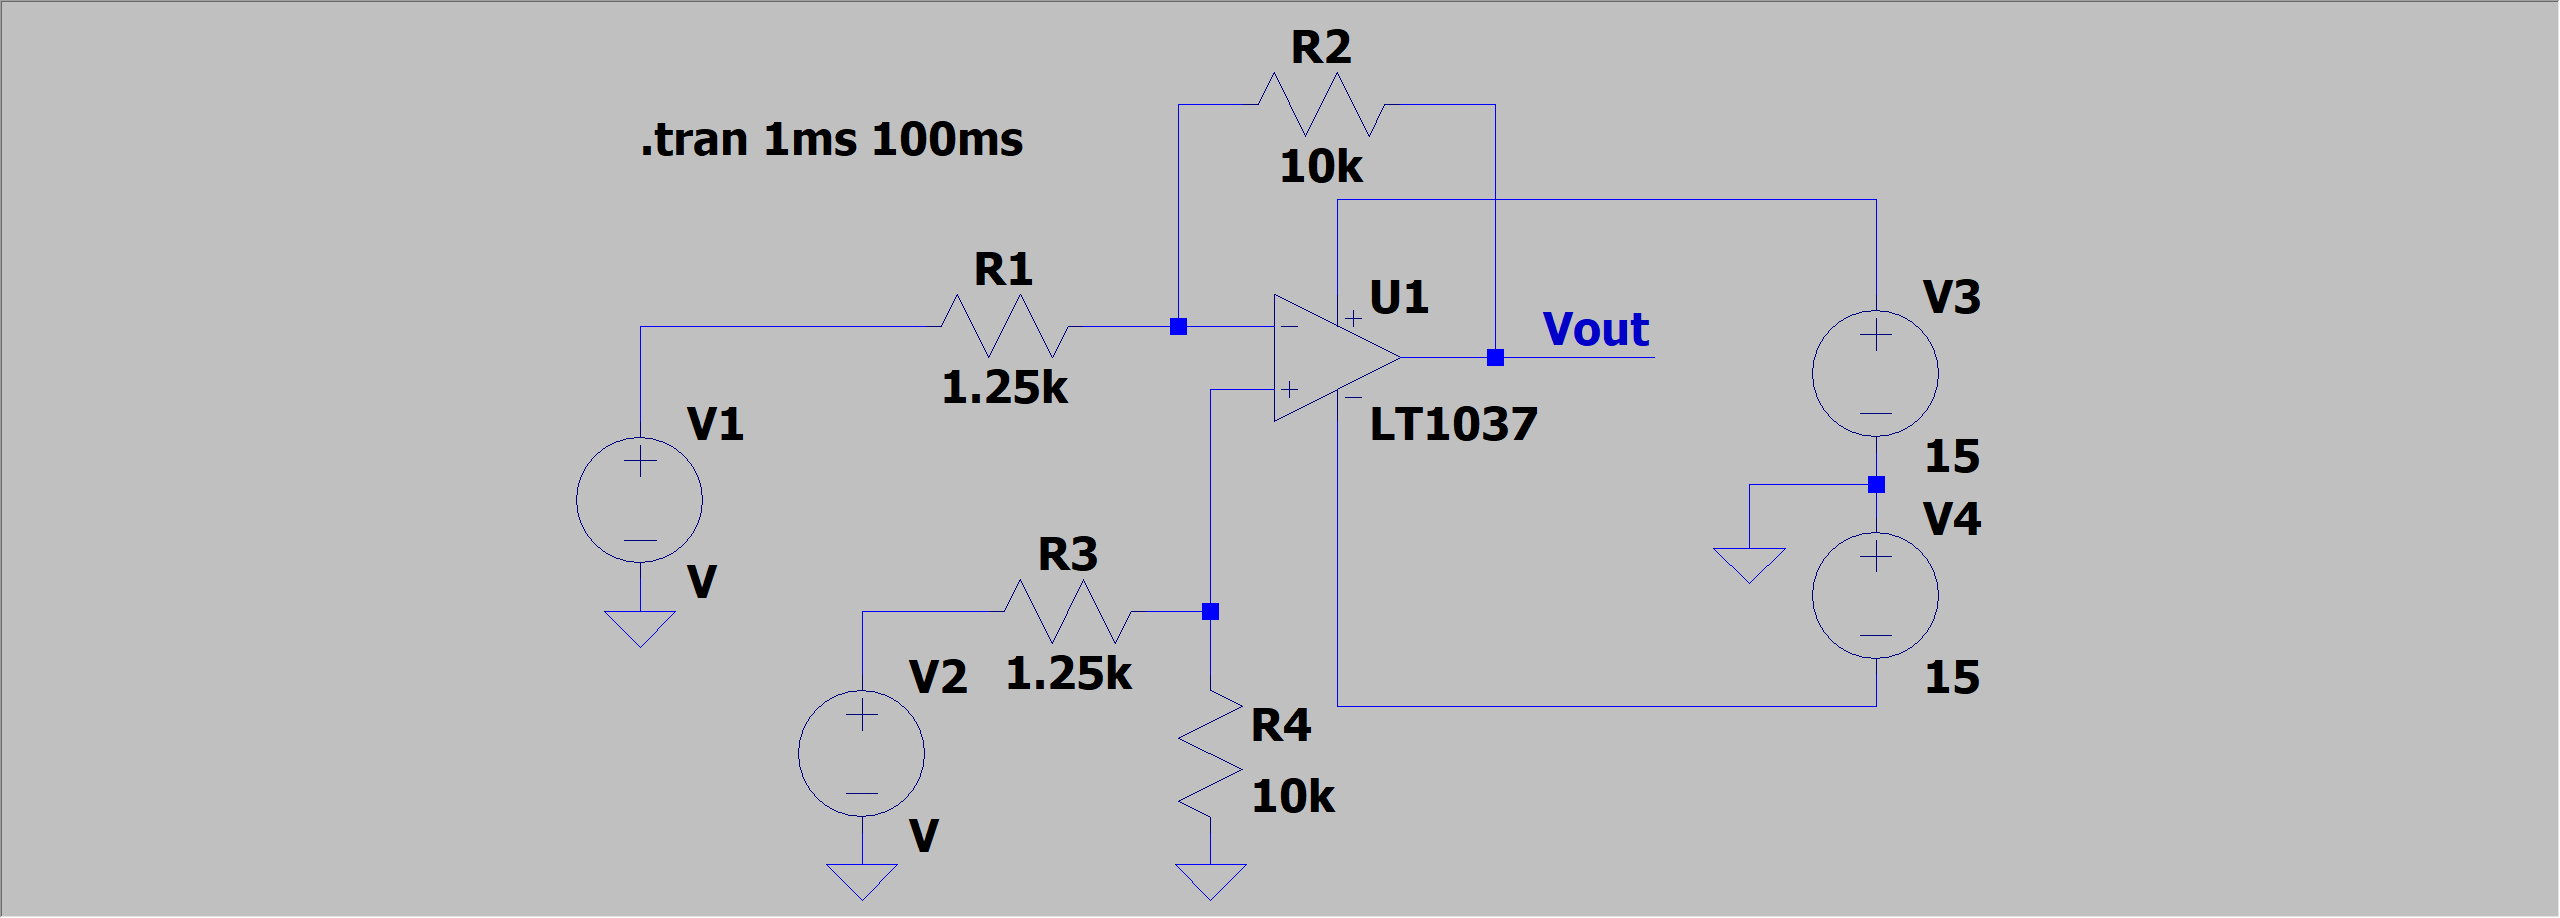
\includegraphics[scale=0.22]{scheme1.png}
        \captionsetup{skip=0pt}
        \caption{Дифференциальный усилитель}
        \label{fig:scheme1}
    \end{figure}


    \subsection{Измерение выходного напряжения при входных напряжениях различной полярности}
    Подаем на V1 отрицательный постоянный ток, на V2 положительный. Измеряем Vout. Считаем
    $U_{\text{вых. теор.}}=R_2/R_1\left( U_2-U_1 \right)$
    \begin{center}
        \begin{tabular}{ | m{6em} | m{3em}| m{3em} | m{3em} | m{3em} | m{3em} | m{3em} | m{3em} | } 
        \hline
        $U_1$, В& $-0.1$ &$-0.3$ &$-0.5$ &$-1$& $-1.5$ & $-0.9$ &$0$\\ 
        \hline
        $U_2$, В& $0.1$ &$0.2$ &$1$ &$0.1$& $0.2$ & $0.9$ &$0.5$\\ 
        \hline
        $U_{\text{вых. эксп.}}$, В& $1.6$ &$4$ &$12$ &$8.8$& $13.59$ & $13.771$ &$4$\\
        \hline
        $U_{\text{вых. теор.}}$, В& $1.6$ &$4$ &$12$ &$8.8$& $13.6$ & $14.4$ &$4$\\
        \hline
        \end{tabular}
    \end{center}
    Почти все результаты совпадают. Видим, что при приближении разницы входных напряжений к значению
    тока, питающего ОУ, деленного на коэффициент усиления ($U_{1,2\,\text{крит.}}=15/8=1.875$ В),
    экспериментальные выходные напряжения отличаются от
    теоретически рассчитаных. У ОУ LT1037 есть ограничения на рабочий диапазон входов,
    он не Rail-to-Rail типа (не может выдать напряжение, равное его питанию).


    Проверим графиком для случая $U_1=-0.1$ В, $U_2=0.1$ В
    \begin{figure}[H]
        \centering
        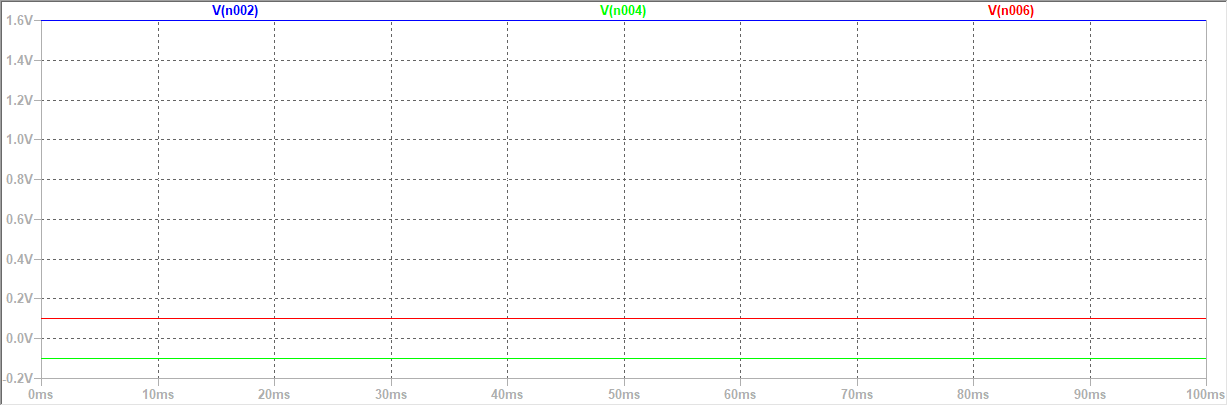
\includegraphics[scale=0.46]{1task_check.png}
        \captionsetup{skip=0pt}
        \caption{Выходное напряжение при $U_1=-0.1$ В, $U_2=0.1$ В}
        \label{fig:1task_check}
    \end{figure}


    \subsection{Влияние синфазной помехи на работу ДУ}
    Подадим одновременно на инвертирующий и неинвертирующий входы ОУ гармонический сигнал SINE(0.1 0.1 1k).
    Схема приведена на рис. \ref{fig:scheme2}.
    Результат приведен на рис. \ref{fig:1task_sine2}
    \begin{figure}[H]
        \centering
        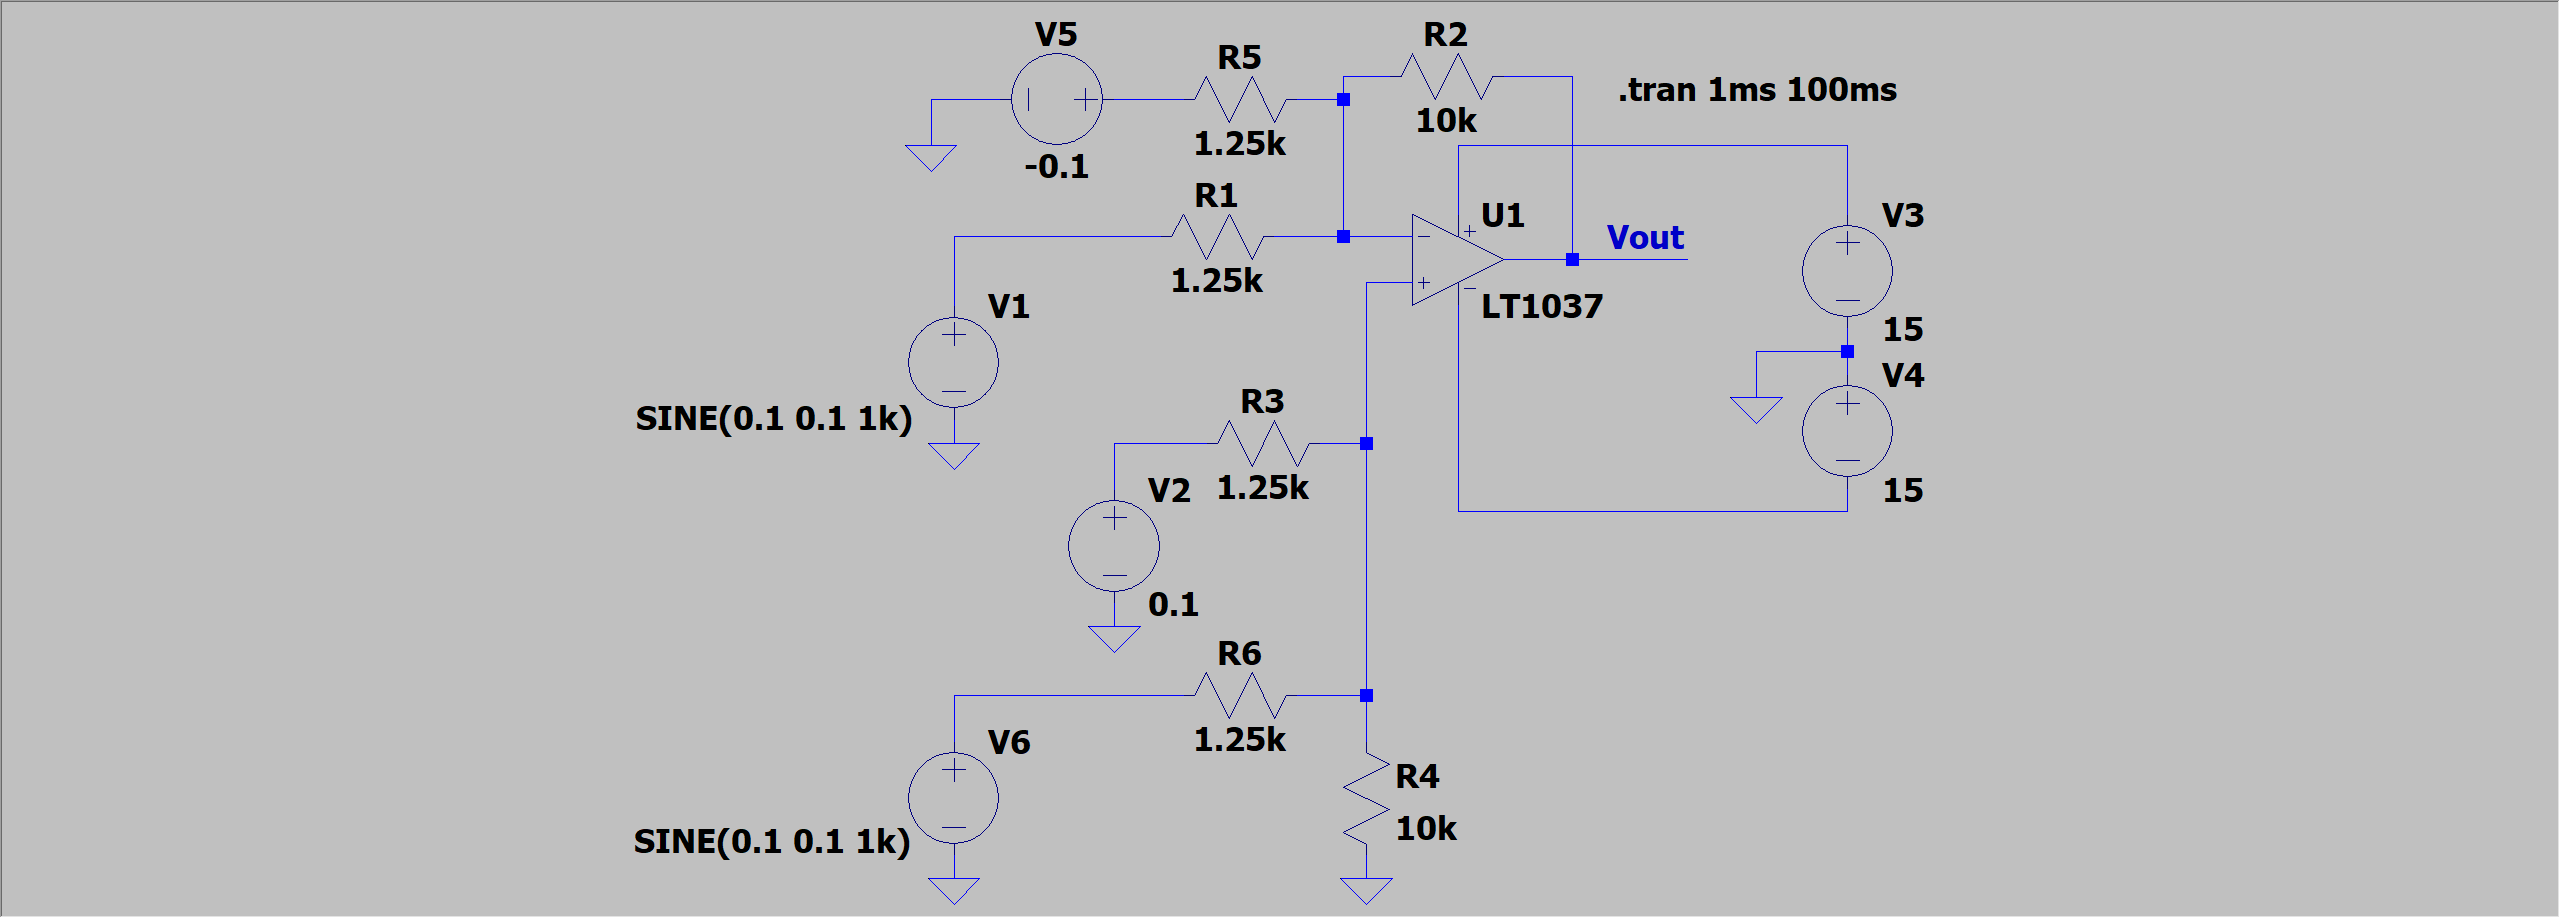
\includegraphics[scale=0.22]{scheme2.png}
        \captionsetup{skip=0pt}
        \caption{Дифференциальный усилитель при имитации воздействия синфазной помехи}
        \label{fig:scheme2}
    \end{figure}
    \begin{figure}[H]
        \centering
        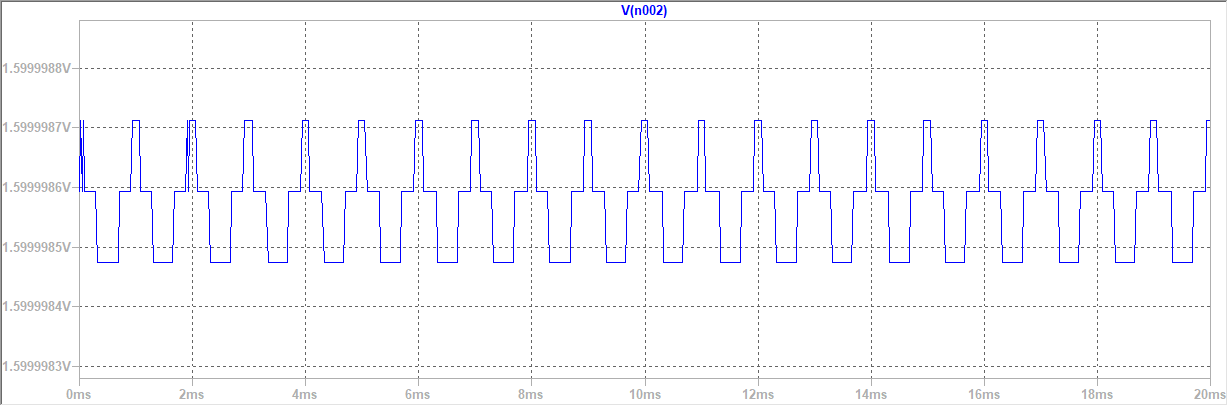
\includegraphics[scale=0.46]{1task_sine2.png}
        \captionsetup{skip=0pt}
        \caption{Выходное напряжение при синфазной помехе}
        \label{fig:1task_sine2}
    \end{figure}
    \noindent Видим, что синфазная помеха почти полностью подавлена, но есть очень маленький остаточный шум.
    Среднее значение $U_{\text{вых. эксп.}}$ по графику соответствует 1.6 В, что совпадает с результатом вычисления
    $U_{\text{вых. теор.}}=8\cdot\left( 0.1-\left( -0.1 \right) \right)=1.6$ В без учета гармонического шума (так как он подавится ДУ).
    В случае идеального ДУ на выходе было бы ровно 1.6 В без помех.


    \subsection{Влияние противофазной помехи на работу ДУ}
    Для имитации противофазной помехи подадим гармонический сигнал SINE(0.1 0.1 1k) на один из входов ОУ.
    Оставим подачу постоянного тока в 0.1 В на оба входа. Схема представлена на рис. \ref{fig:scheme3}. Результат представлен на рис. \ref{fig:1task_sine1}
    \begin{figure}[H]
        \centering
        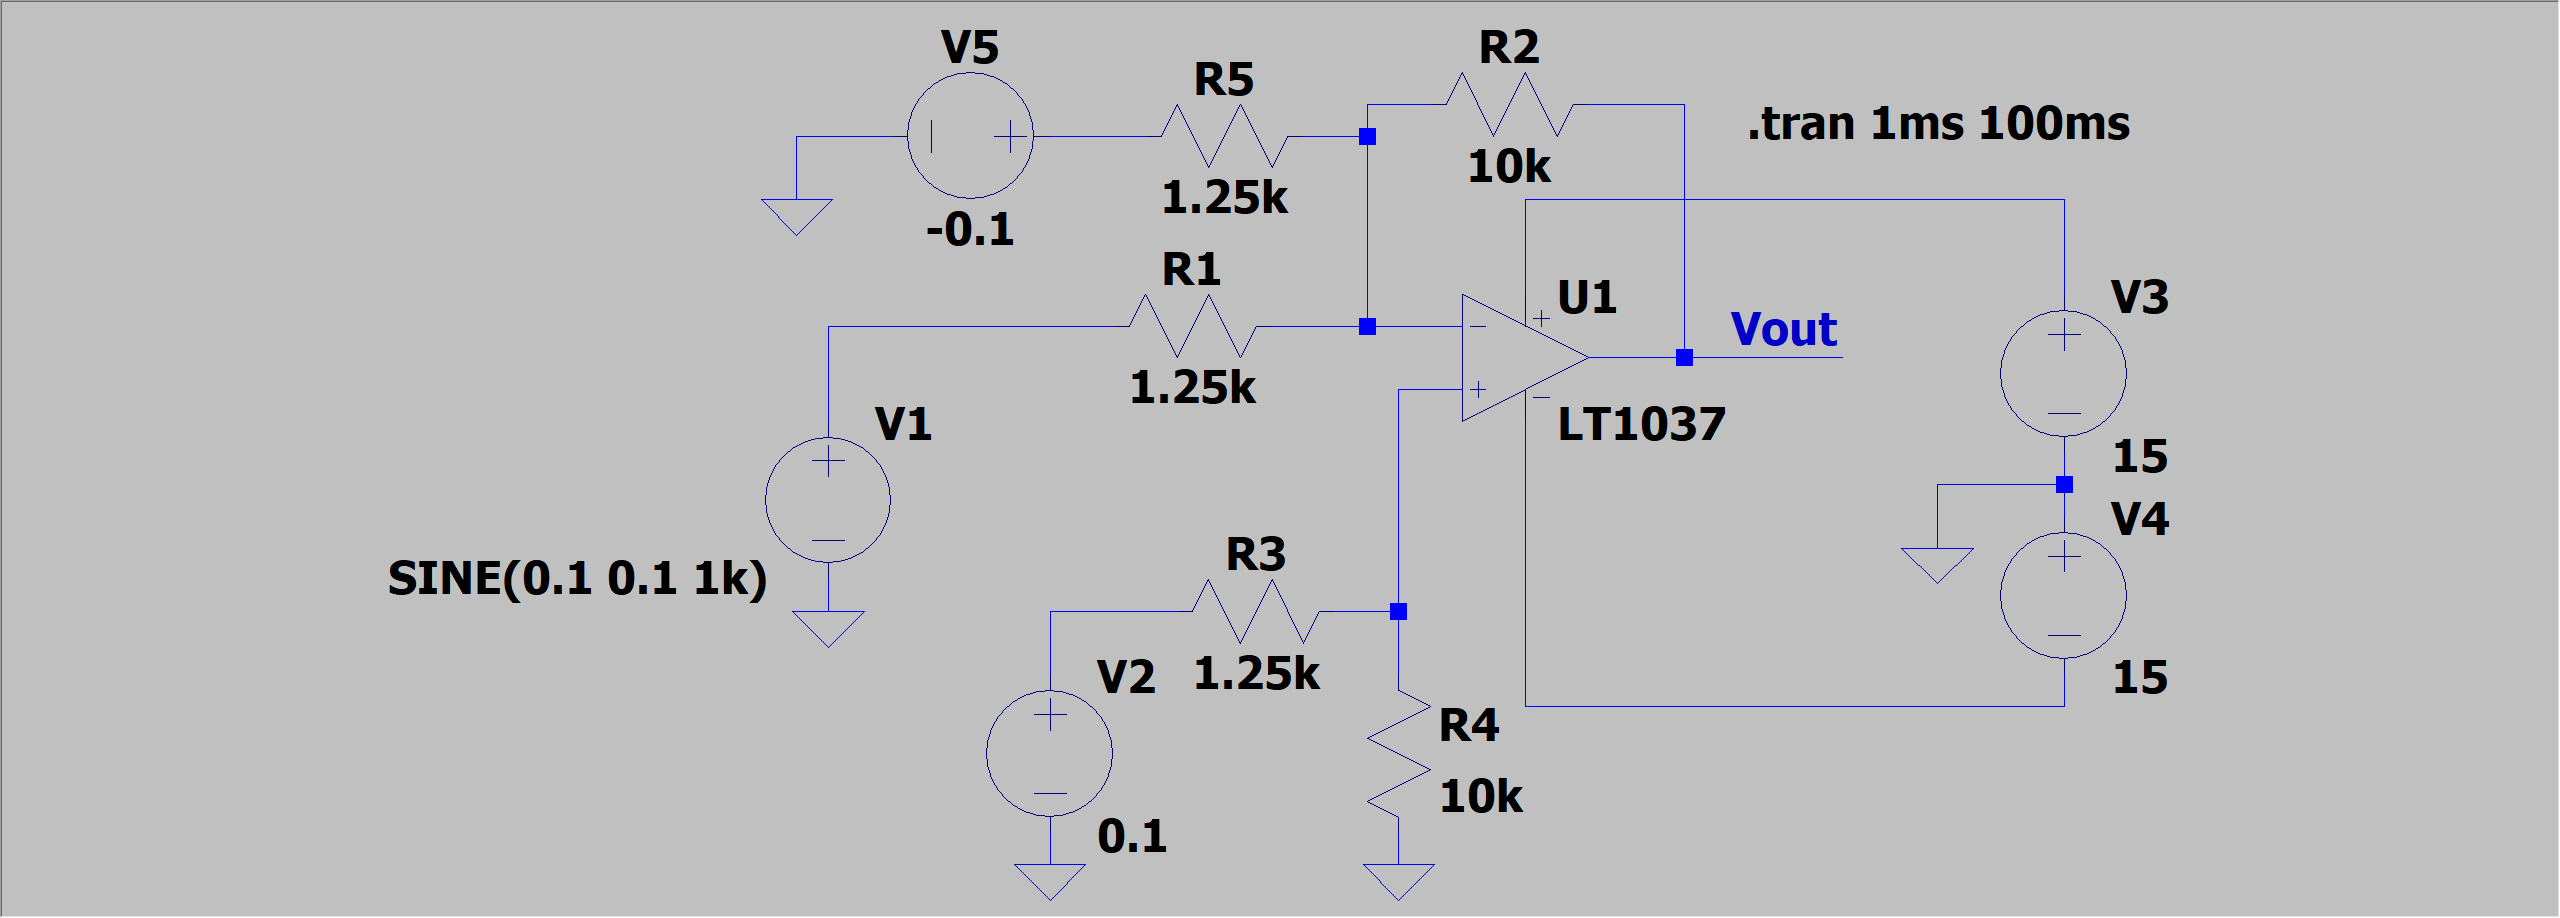
\includegraphics[scale=0.22]{scheme3.png}
        \captionsetup{skip=0pt}
        \caption{Дифференциальный усилитель при имитации воздействия противофазной помехи}
        \label{fig:scheme3}
    \end{figure}
    \begin{figure}[H]
        \centering
        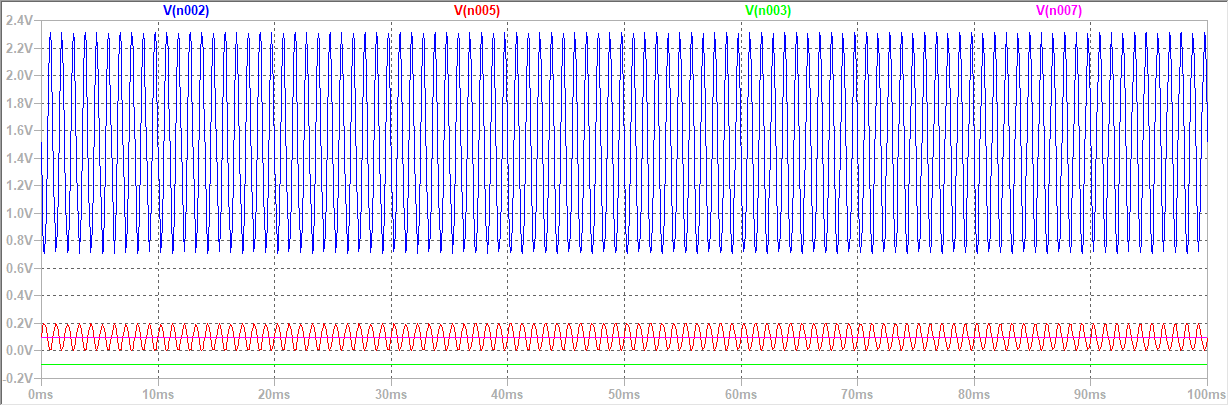
\includegraphics[scale=0.46]{1task_sine1.png}
        \captionsetup{skip=0pt}
        \caption{Выходное напряжение при противофазной помехе}
        \label{fig:1task_sine1}
    \end{figure}
    \noindent ОУ усилил разницу между $U_1,U_2$. Синусоида сместилась вверх и увеличила амплитуду. Среднее значение 
    выходного напряжения составляет 1.5111 В. Это близко к значению $U_{\text{вых. теор.}}=1.6$ В, вычисленному в пункте с синфазной помехой.


    \section{ОУ в режиме суммирования постоянных сигналов}
    \subsection{Схема инвертирующего сумматора на ОУ}
    Соберем схему инвертирующего сумматора на ОУ AD549
    \begin{figure}[H]
        \centering
        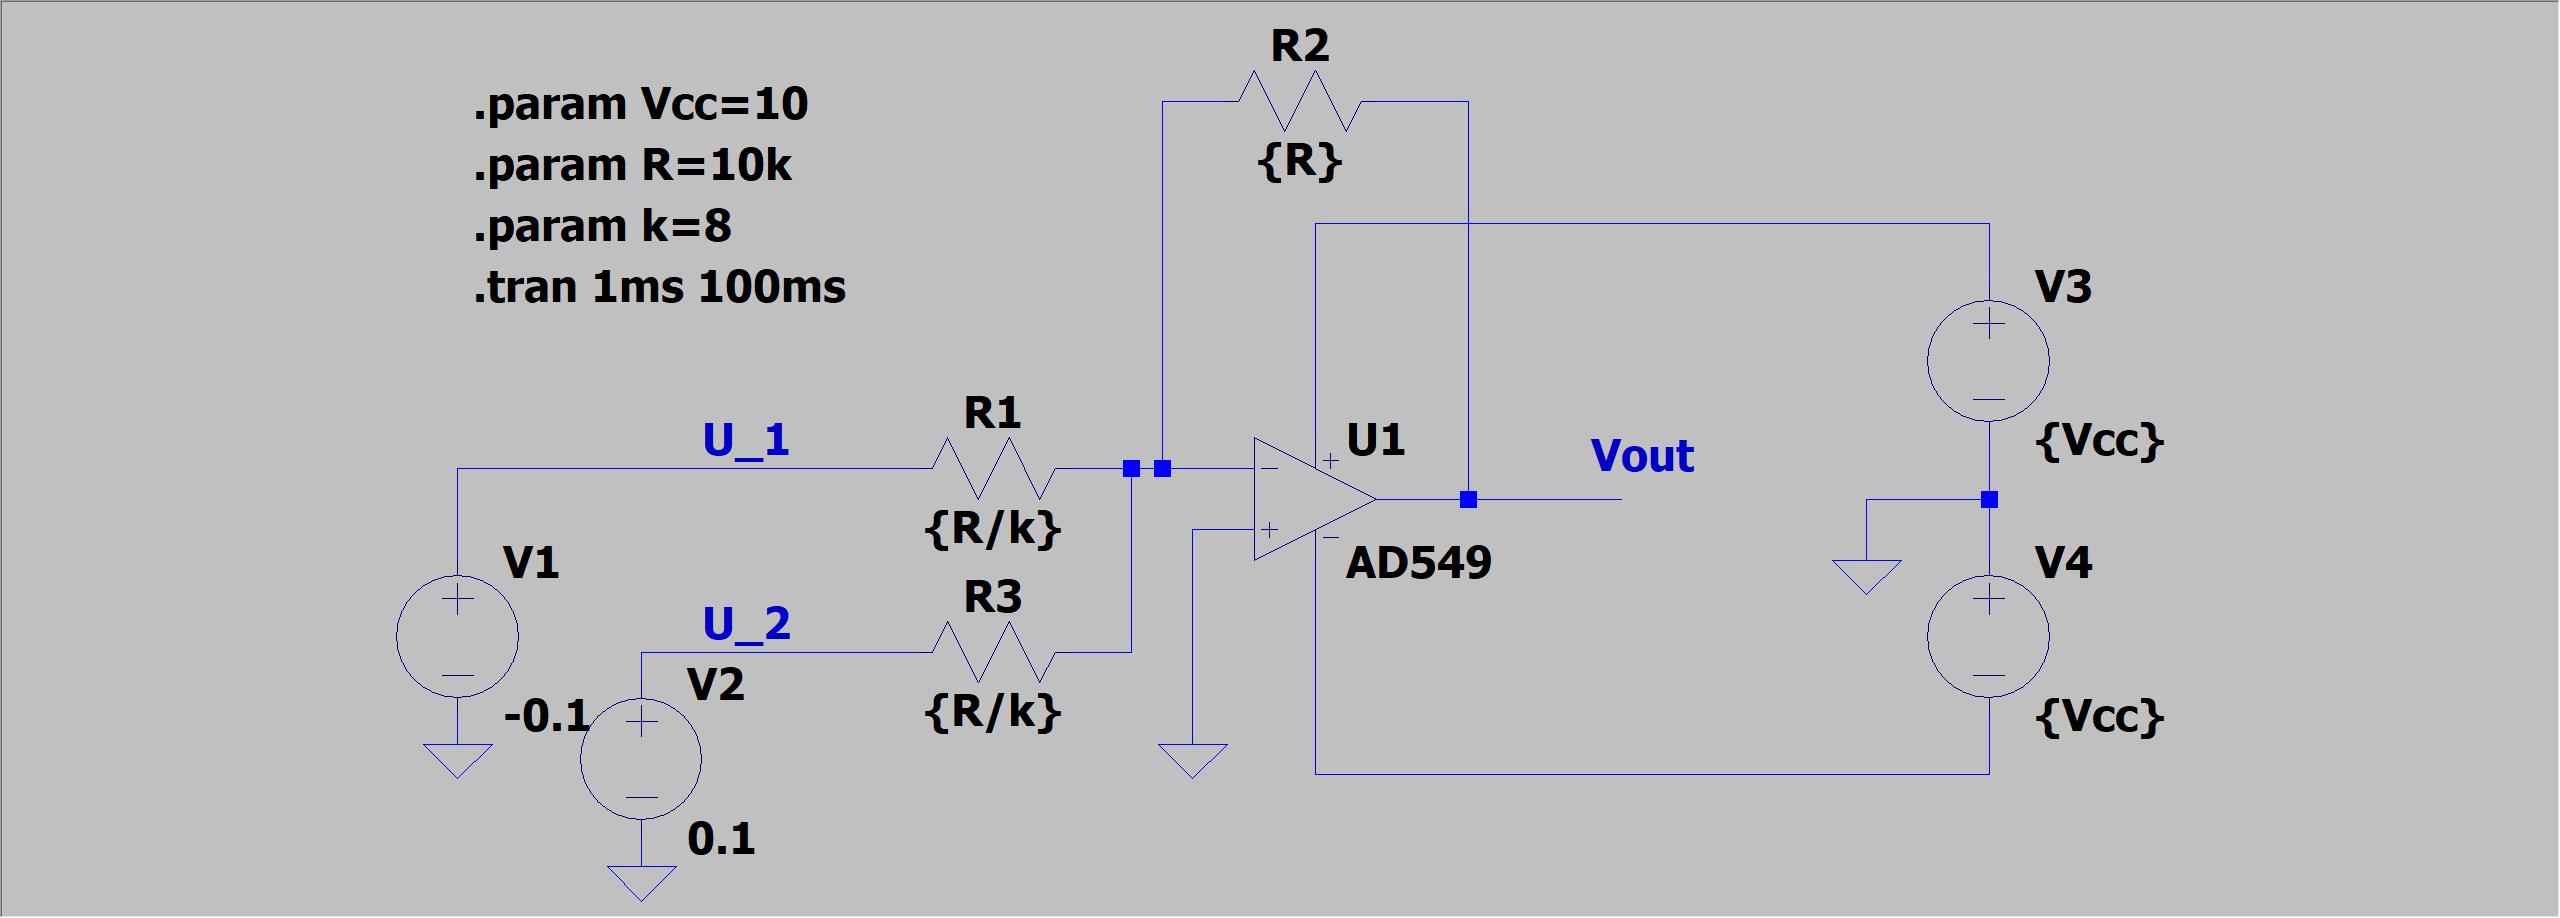
\includegraphics[scale=0.22]{scheme4.png}
        \captionsetup{skip=0pt}
        \caption{Инвертирующий сумматор на ОУ}
        \label{fig:scheme4}
    \end{figure}

    
    \subsection{Измерение выходного напряжения при входных напряжениях различной полярности}
    Подаем на V1 отрицательный постоянный ток, на V2 положительный. Измеряем Vout. Считаем
    $U_{\text{вых. теор.}}=-\left( \left(R_2/R_1\right)U_1+\left(R_2/R_3\right)U_2 \right),\ R_2/R_1=R_2/R_3=8$
    \begin{center}
        \begin{tabular}{ | m{5.5em} | m{4em}| m{3.5em} | m{4em} | m{3em} | m{3em} | m{3em} | m{4em} | } 
        \hline
        $U_1$, В& $-0.1$ &$-0.3$ &$-0.5$ &$-1$& $-1.5$ & $-1.25$ &$0$\\ 
        \hline
        $U_2$, В& $0.1$ &$0.2$ &$1$ &$0.1$& $1$ & $0.05$ &$0.5$\\ 
        \hline
        $U_{\text{вых. эксп.}}$, В& $-6.1023\cdot10^{-6}$ &$0.79998$ &$-3.9999$ &$7.1999$& $3.9999$ & $8.2148$ &$-3.9999$\\
        \hline
        $U_{\text{вых. теор.}}$, В& $0$ &$0.8$ &$-4$ &$7.2$& $4$ & $9.6$ &$-4$\\
        \hline
        \end{tabular}
    \end{center}
    Как видим экспериментальные и теоретические значения почти совпали.
    При приближении разности $U_1,U_2$ к $U_{1,2\,\text{крит.}}=10/8=1.25$ В
    экспериментальные значения начинают отставать аналогично заданию с ДУ.


    Проверим графиком для случая $U_1=-0.1$ В, $U_2=0.1$ В
    \begin{figure}[H]
        \centering
        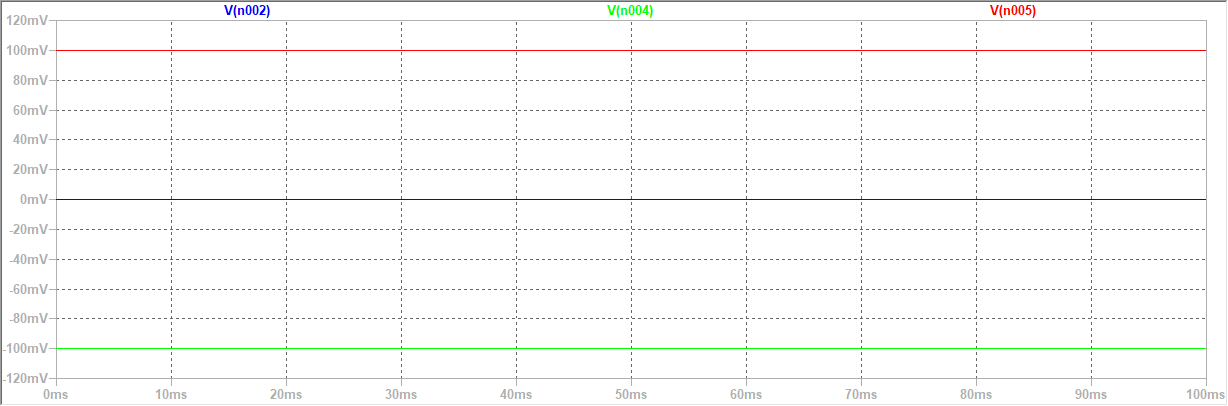
\includegraphics[scale=0.46]{scheme4_check.png}
        \captionsetup{skip=0pt}
        \caption{Выходное напряжение при $U_1=-0.1$ В, $U_2=0.1$ В}
        \label{fig:scheme4_check}
    \end{figure}


    \section{Неинвертирующий сумматор для двух сигналов на ОУ}
    \subsection{Схема неинвертирующего сумматора на ОУ}
    Соберем схему неинвертирующего сумматора для двух сигналов с ОУ,
    обеспечивающего суммирование двух сигналов с заданными весовыми
    коэффициентами $K_1,K_2$
    \begin{figure}[H]
        \centering
        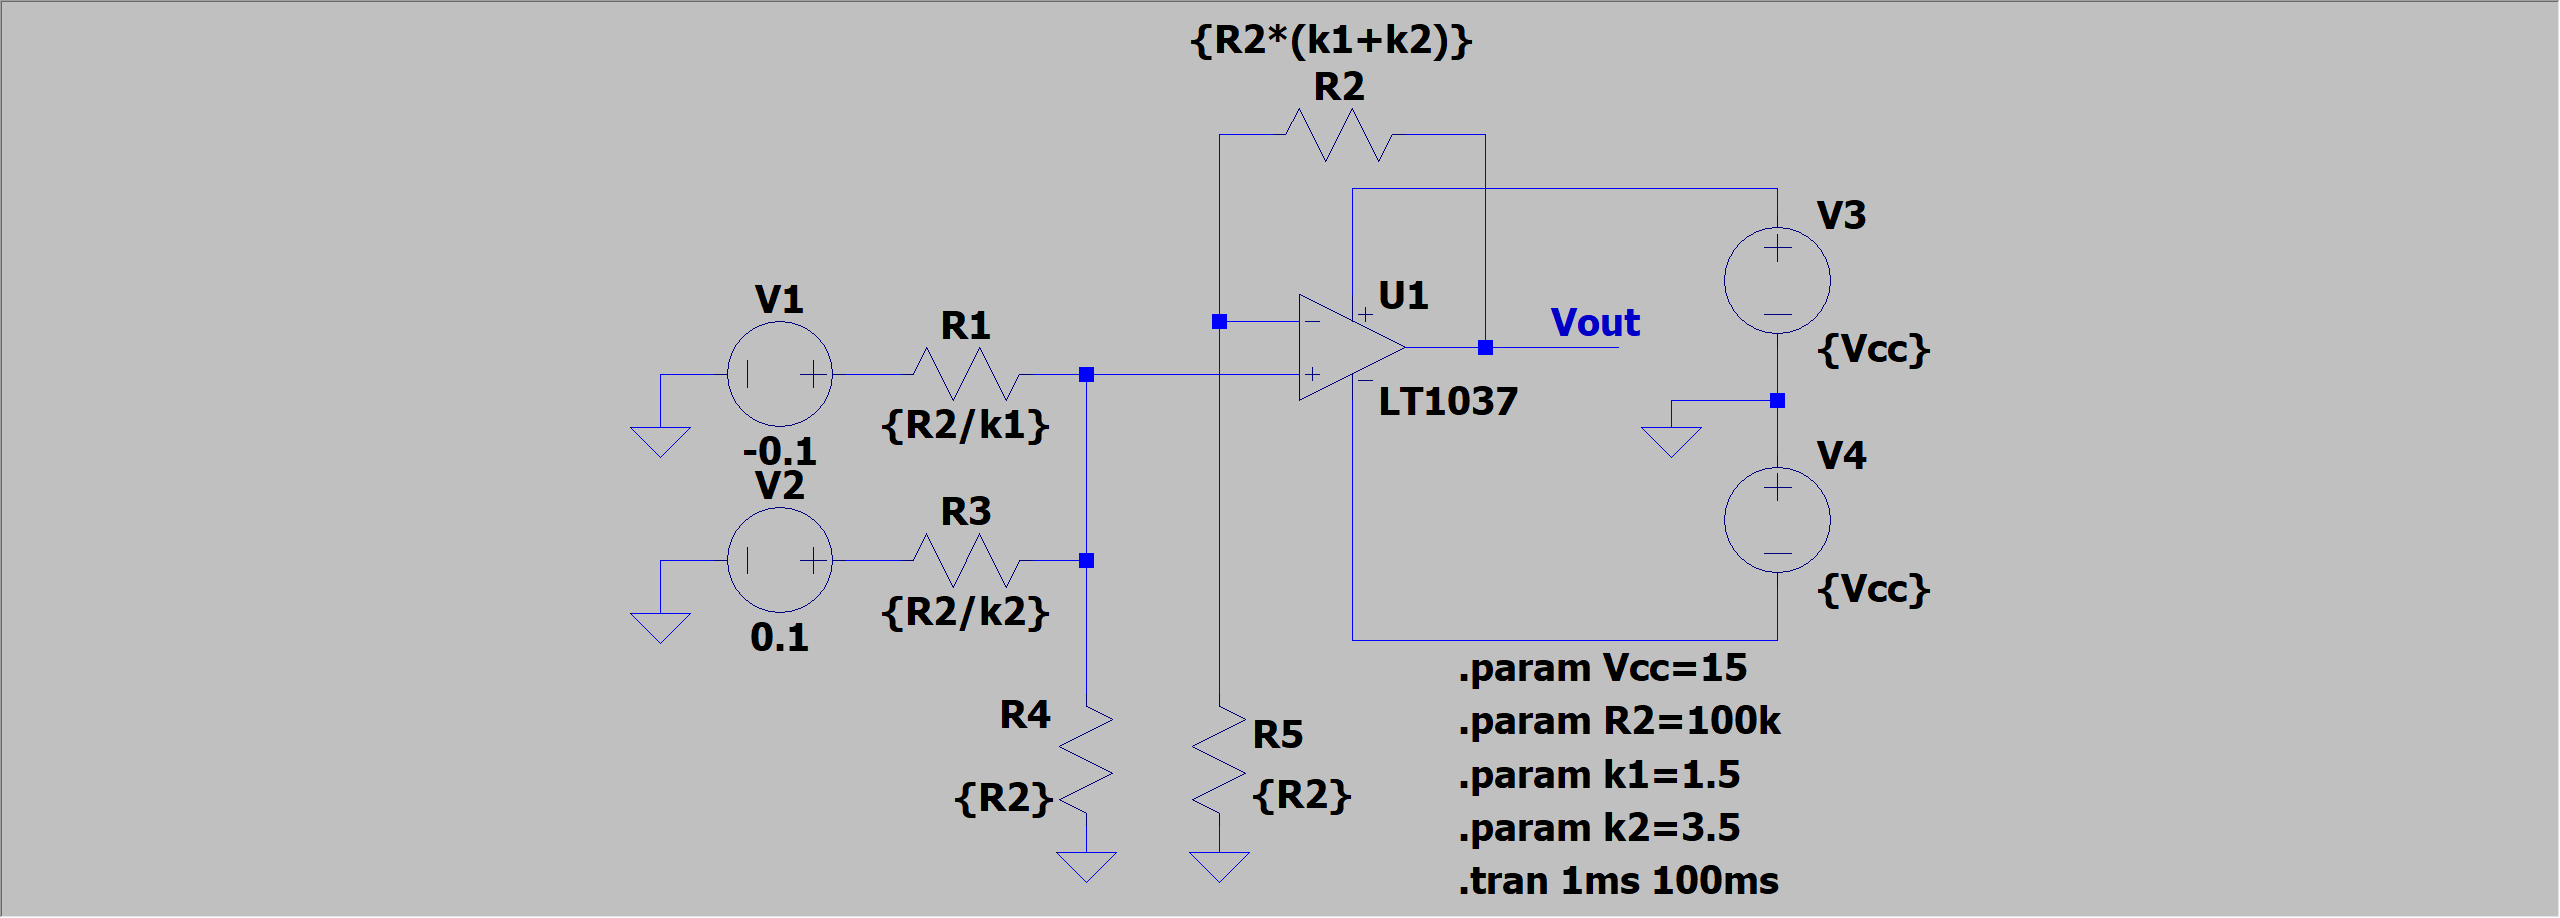
\includegraphics[scale=0.22]{scheme5.png}
        \captionsetup{skip=0pt}
        \caption{Неинвертирующий сумматор на ОУ}
        \label{fig:scheme5}
    \end{figure}


    \subsection{Измерение выходного напряжения при входных напряжениях различной полярности}
    Подаем на V1 отрицательный постоянный ток, на V2 положительный. Измеряем Vout. Считаем
    $U_{\text{вых. теор.}}=\left(R_4/R_1\right)U_1+\left(R_4/R_3\right)U_2=K_1U_1+K_2U_2,\ R_2/R_5=K_1+K_2,\ R_5=R_4=100$ кОм
    \begin{center}
        \begin{tabular}{ | m{5.5em} | m{2.5em}| m{2.5em} | m{2.5em} | m{3em} | m{3em} | m{2.5em} | m{2.5em} | m{2.5em} | } 
        \hline
        $U_1$, В& $-0.1$ &$-0.3$ &$-0.5$ &$-1$& $-1.5$ & $-2$ & $-3$ &$0$\\ 
        \hline
        $U_2$, В& $0.1$ &$0.2$ &$1$ &$0.1$& $0.2$ & $3$ &$5$ &$0.5$\\ 
        \hline
        $U_{\text{вых. эксп.}}$, В& $0.2$ &$0.25$ &$2.75$ &$-1.15$& $-1.55$ & $7.5$ &$13$ &$1.75$\\
        \hline
        $U_{\text{вых. теор.}}$, В& $0.2$ &$0.25$ &$2.75$ &$-1.15$& $-1.55$ & $7.5$& $13$ &$1.75$\\
        \hline
        \end{tabular}
    \end{center}
    Видим, что экспериментальные и теоретические значения совпадают.


    Проверим графиком для случая $U_1=-0.1$ В, $U_2=0.1$ В
    \begin{figure}[H]
        \centering
        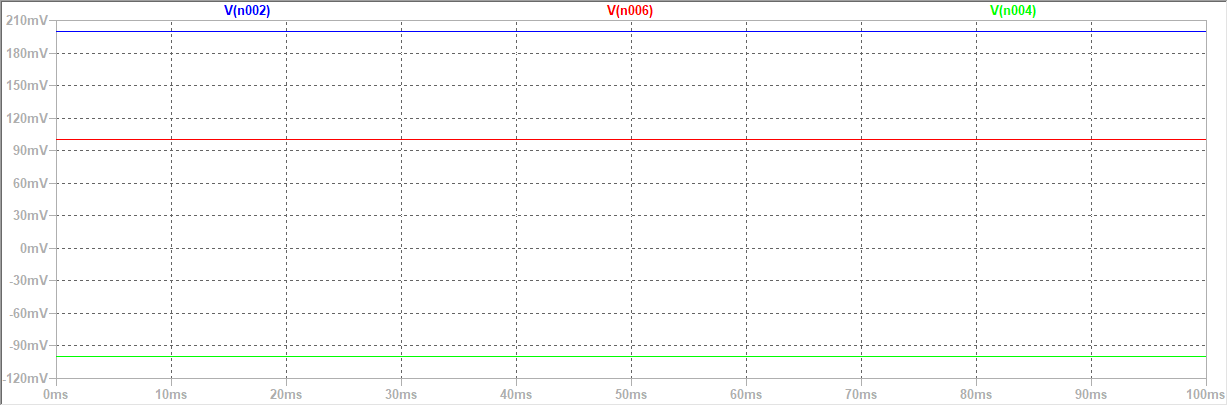
\includegraphics[scale=0.46]{scheme5_check.png}
        \captionsetup{skip=0pt}
        \caption{Выходное напряжение при $U_1=-0.1$ В, $U_2=0.1$ В}
        \label{fig:scheme5_check}
    \end{figure}


    \section{Интегратор на ОУ}
    Соберем схему интегратора на ОУ. Для R1 зададим стандартное значение 100 кОм.
    Интегратор работает на частоте $f_i=1$ кГц. Пусть минимальное и максимальное
    значение рабочей частоты будет $f_{min}=0.01f_i,\ f_{max}=100f_i$. Рассчитаем C1
    $$
    C_1=\dfrac{1}{2\pi f_i R_1}=\dfrac{1}{2\pi\cdot10^3\cdot100\cdot10^3}=1.6\text{ нФ}
    $$
    Рассчитаем R2
    $$
    R_2=\dfrac{1}{2\pi C_1 f_{min}/10}=\dfrac{1}{2\pi\cdot1.6\cdot10^{-9}}=99471839.4324346\text{ Ом}
    $$
    Возьмем $R_2$ больше полученного значения -- $R_2=100$ МОм.
    
    
    Рекомендуется использовать ОУ с полосой пропускания в 10 раз большей, чем требуемая максимальная
    частота интегратора. Проверим:
    $$
    f_{max,\,\text{LT1037}}=2.5\text{ МГц},\ f_{max}=100f_i=100\text{ кГц},\ f_{max,\text{ реком.}}=10f_{max}=1\text{ МГц}
    $$
    $$
    f_{max,\,\text{LT1037}}=2.5\text{ МГц}>f_{max,\text{ реком.}}=1\text{ МГц}
    $$


    \subsection{Схема идеального интегратора на ОУ}
    Построим схему идеального интегратора с учетом всех вычислений
    \begin{figure}[H]
        \centering
        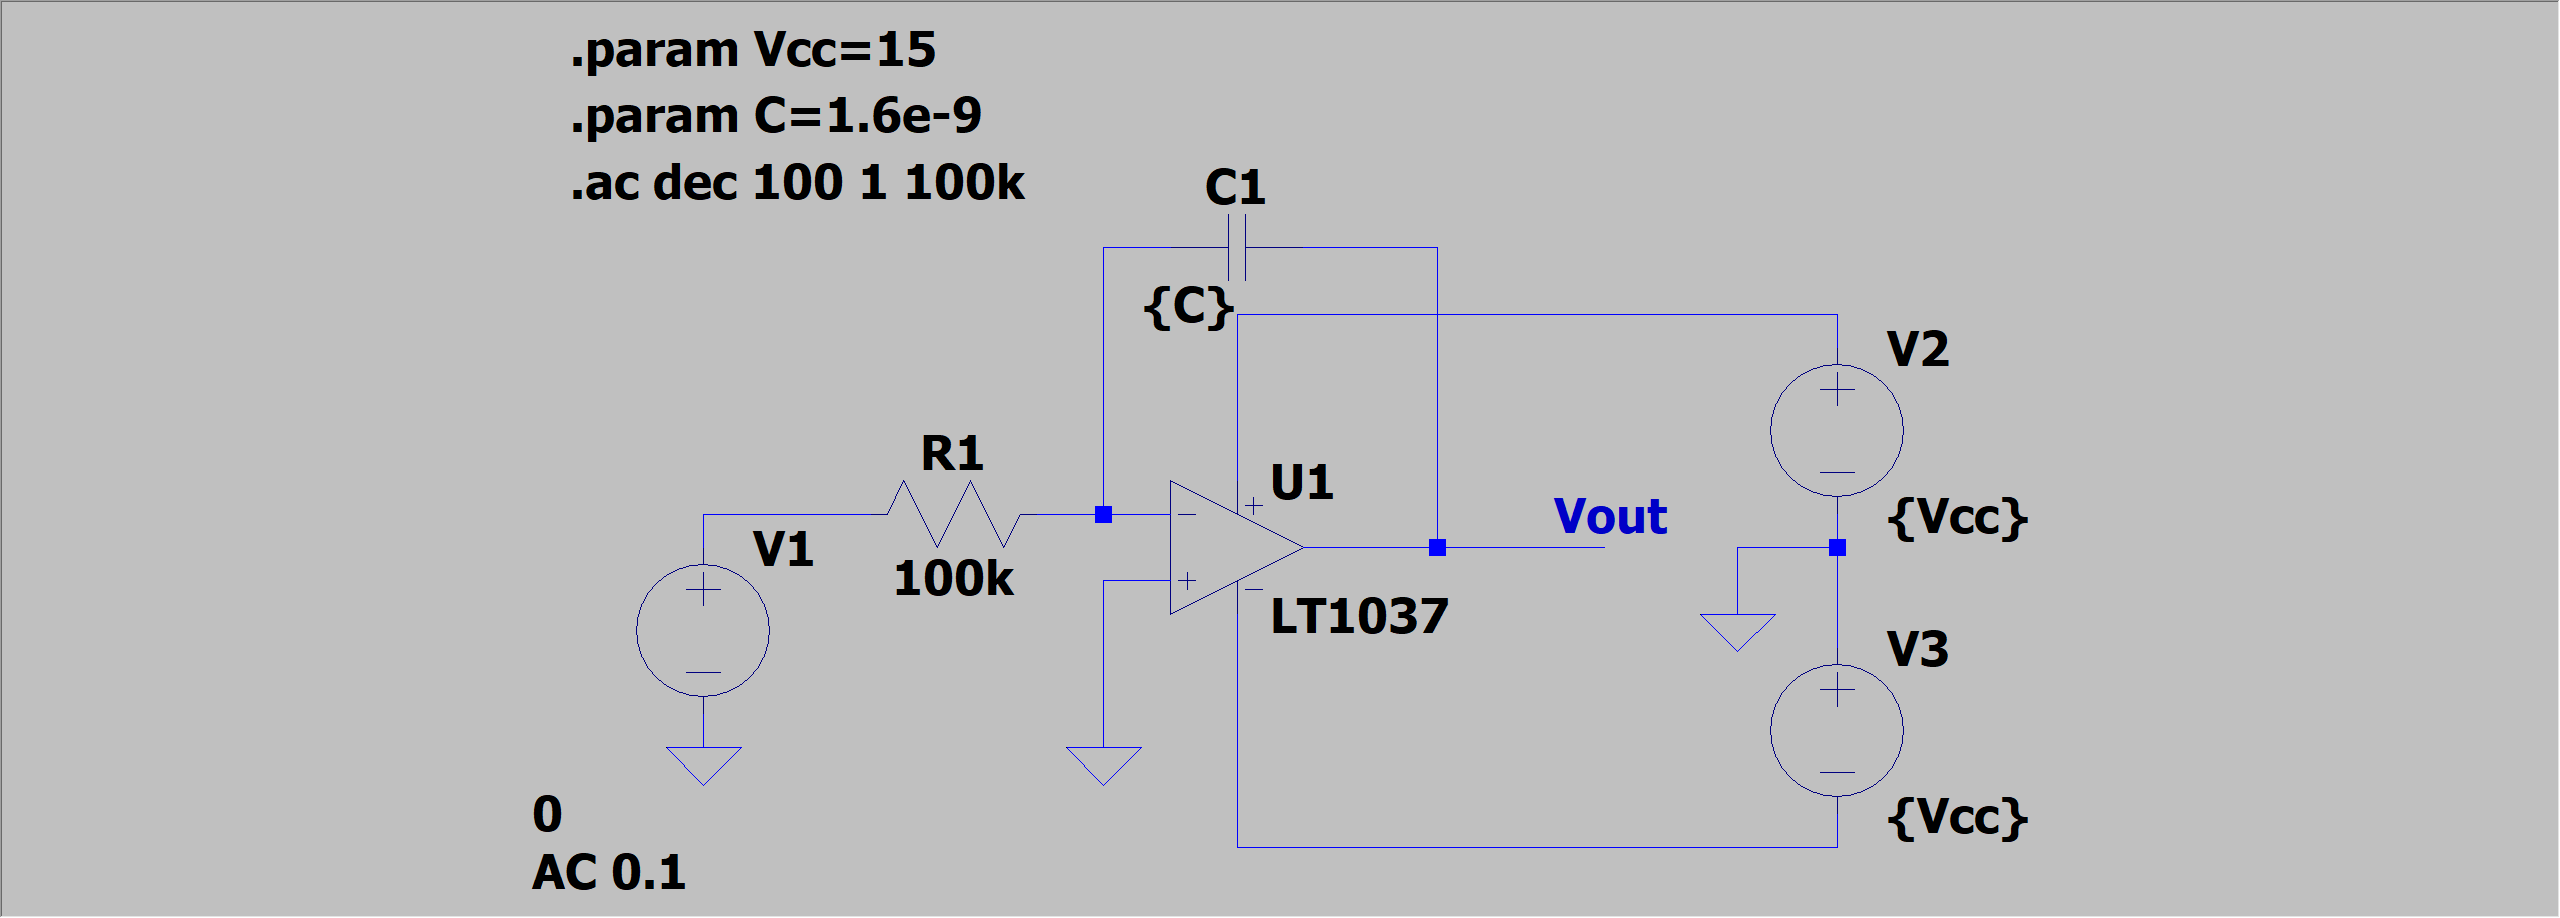
\includegraphics[scale=0.22]{scheme6.png}
        \captionsetup{skip=0pt}
        \caption{Идеальный интегратор на ОУ}
        \label{fig:scheme6}
    \end{figure}


    \subsection{Схема реального интегратора на ОУ}
    Построим схему реального интегратора с учетом всех вычислений
    \begin{figure}[H]
        \centering
        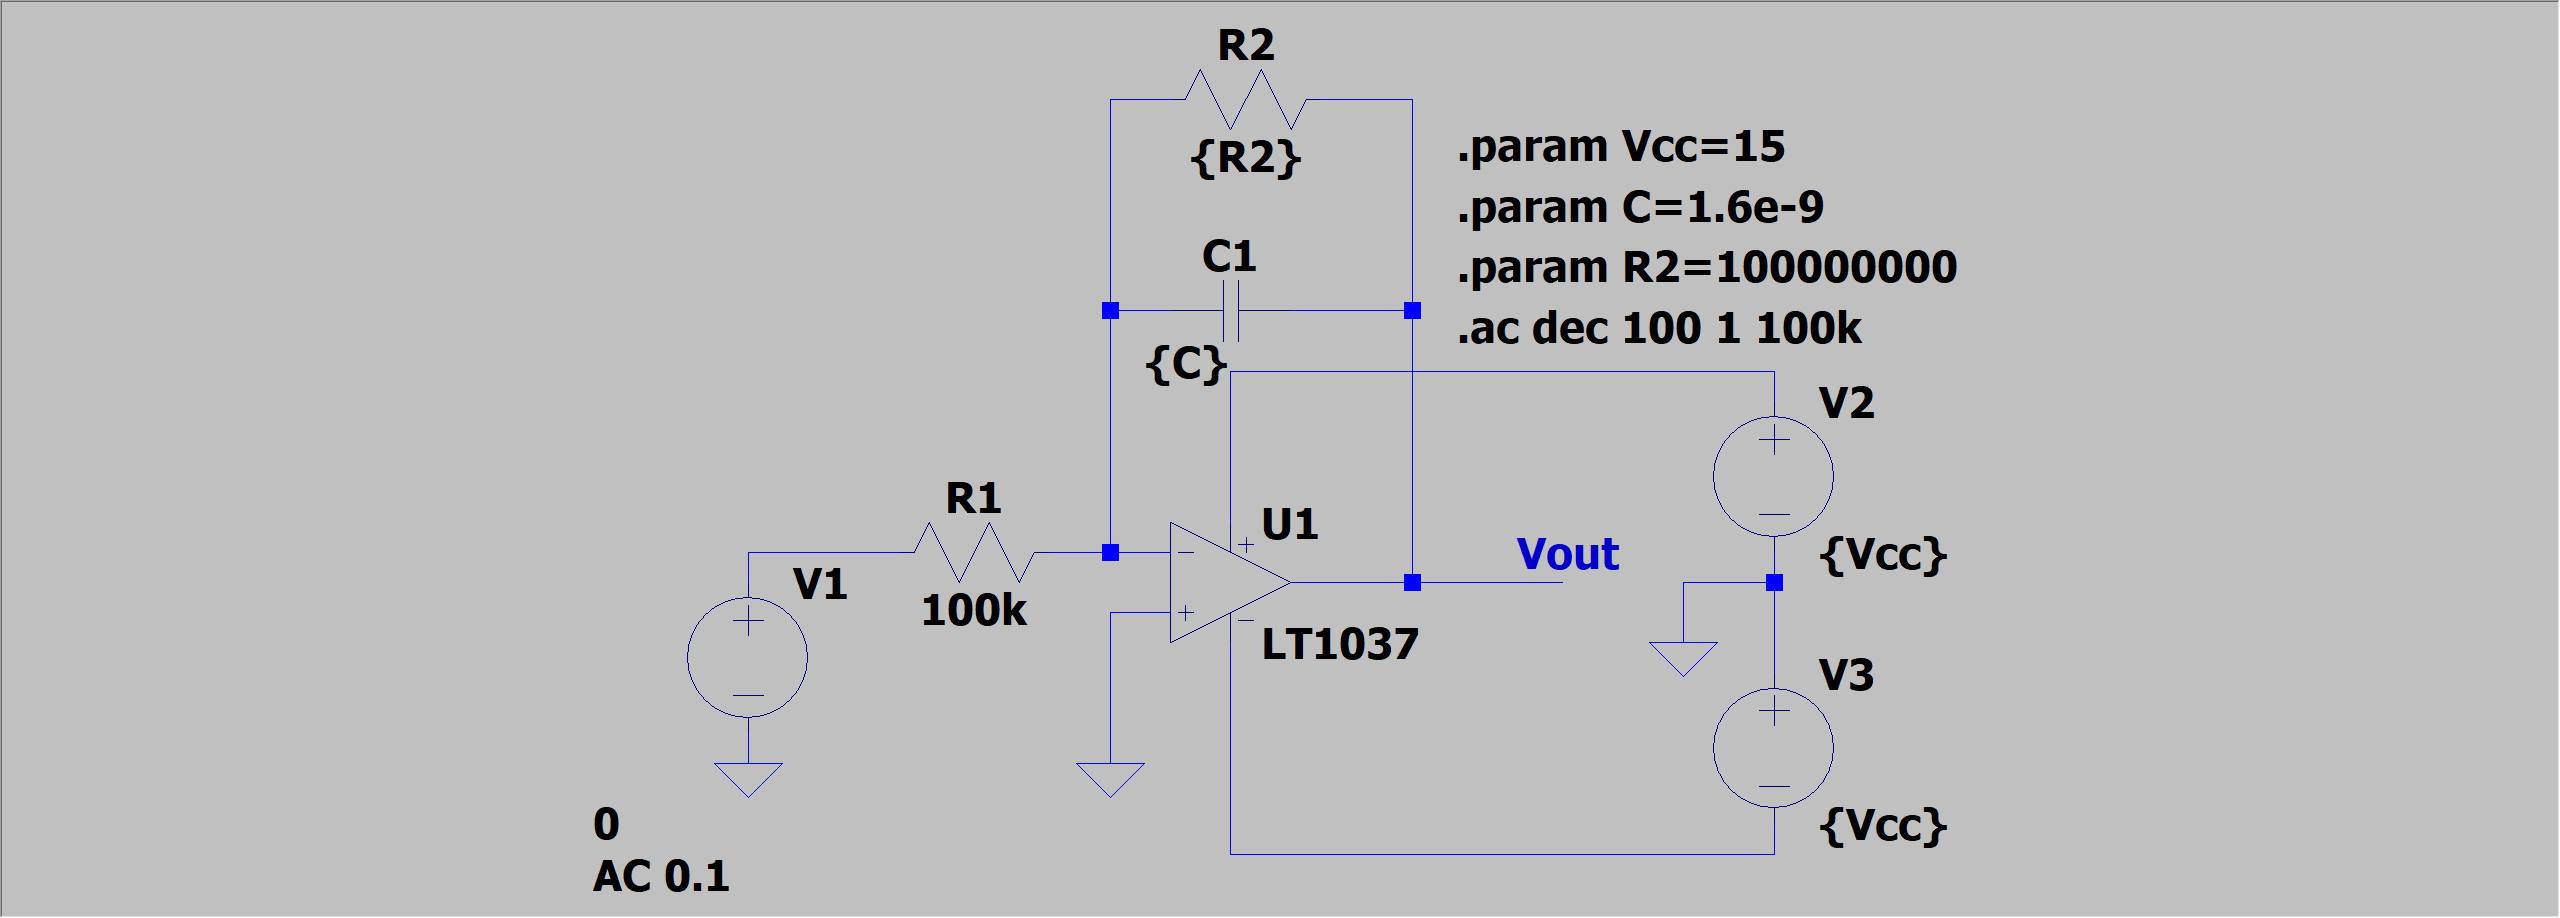
\includegraphics[scale=0.22]{scheme7.png}
        \captionsetup{skip=0pt}
        \caption{Реальный интегратор на ОУ}
        \label{fig:scheme7}
    \end{figure}


    \subsection{Частотная характеристика интегратора}
    Подадим на вход гармонический сигнал, не искажающий выходной сигнал (AC 0.1). Идеальный
    интегратор представлен на рис. \ref{fig:3task_ideal_int}, реальный на \ref{fig:3task_real_int}
    \begin{figure}[H]
        \centering
        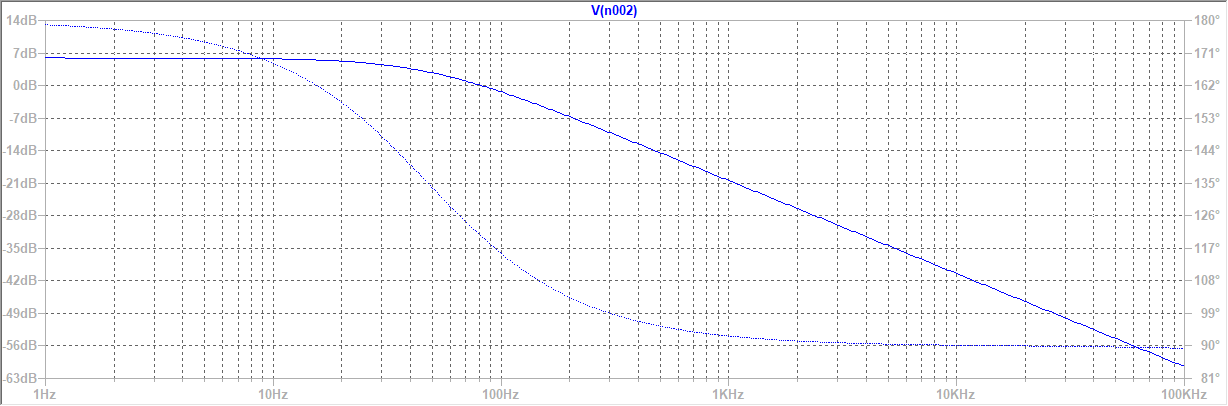
\includegraphics[scale=0.46]{3task_ideal_int.png}
        \captionsetup{skip=0pt}
        \caption{Частотная характеристика идеального интегратора}
        \label{fig:3task_ideal_int}
    \end{figure}
    \begin{figure}[H]
        \centering
        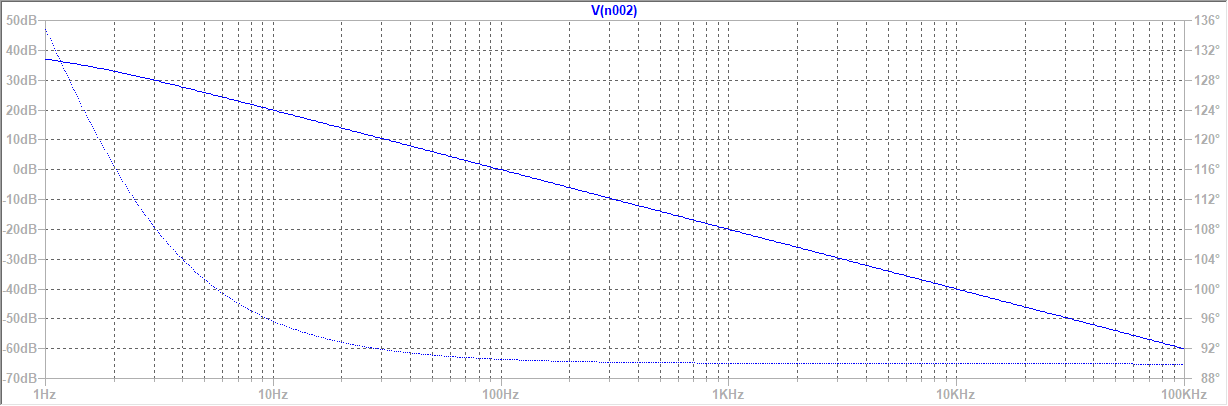
\includegraphics[scale=0.46]{3task_real_int.png}
        \captionsetup{skip=0pt}
        \caption{Частотная характеристика реального интегратора}
        \label{fig:3task_real_int}
    \end{figure}
    \noindent Посчитаем частоту среза
    $$
    f_{\text{срез.}}=\dfrac{1}{2\pi R_2 C_1}=\dfrac{1}{2\pi\cdot10^8\cdot1.6\cdot10^{-9}}=0.9947183943\text{ Гц}
    $$
    То есть реальный интегратор перестает быть идеальным уже около 1 Гц, дальше ведет себя ближе к обычному усилителю.


    \subsection{Вид выходного сигнала при разных входных сигналах}
    Проверим экспериментально вид выходного сигнала для следующих
    входных сигналов (параметры могут меняться в зависимости от задания): 
    \begin{itemize}
        \item синусоидальный SINE(0.1 0.1 1k)
        \item треугольный PULSE(0 10 0.01ms .5m .5m 1e-10 1m 1000)
        \item прямоугольный PULSE(0 10 0.01ms 10p 10p 0.1ms 0.2ms)
    \end{itemize}
    Результаты представлены на рис. \ref{fig:3task_ideal_sine}--\ref{fig:3task_real_rect}
    \begin{figure}[H]
        \centering
        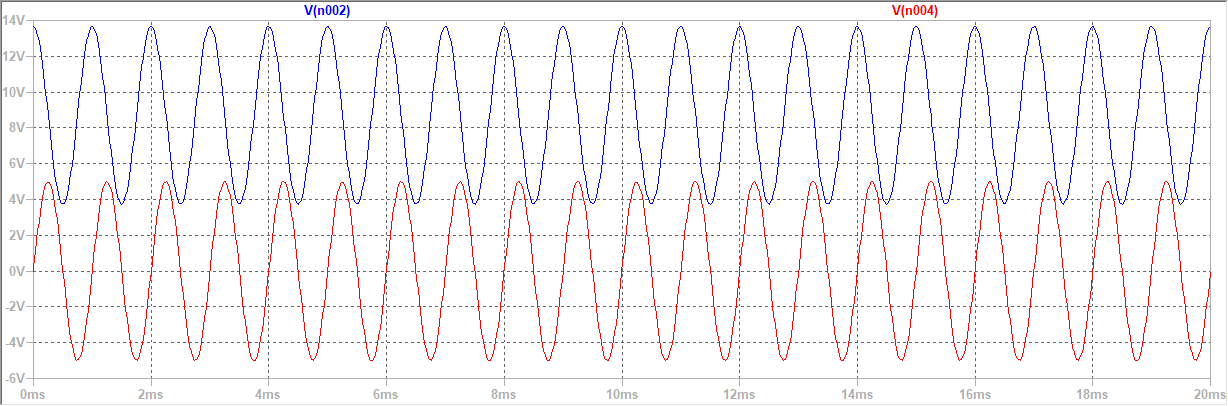
\includegraphics[scale=0.46]{3task_ideal_sine.png}
        \captionsetup{skip=0pt}
        \caption{Синусоидальный сигнал, идеальный интегратор}
        \label{fig:3task_ideal_sine}
    \end{figure}
    \begin{figure}[H]
        \centering
        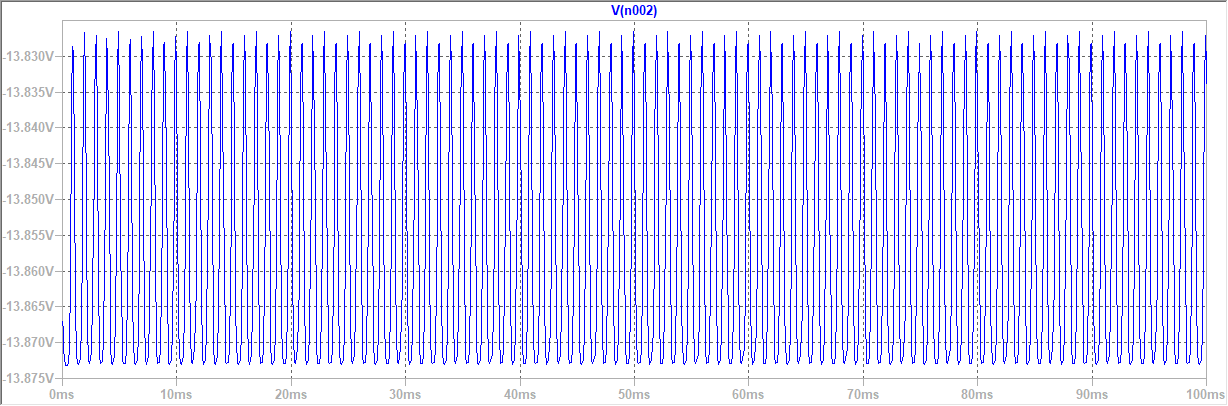
\includegraphics[scale=0.46]{3task_real_sine.png}
        \captionsetup{skip=0pt}
        \caption{Синусоидальный сигнал, реальный интегратор}
        \label{fig:3task_real_sine}
    \end{figure}
    \begin{figure}[H]
        \centering
        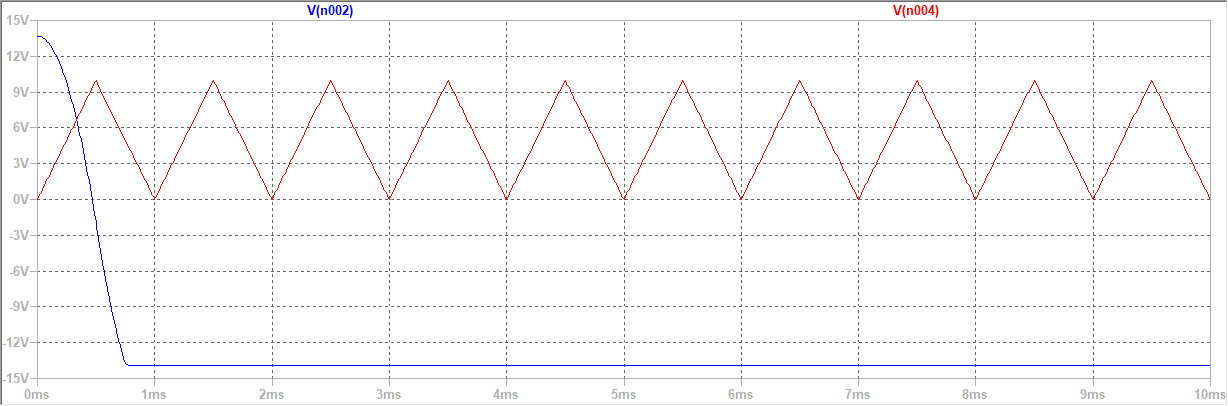
\includegraphics[scale=0.46]{3task_ideal_triangle.png}
        \captionsetup{skip=0pt}
        \caption{Треугольный сигнал, идеальный интегратор}
        \label{fig:3task_ideal_triangle}
    \end{figure}
    \begin{figure}[H]
        \centering
        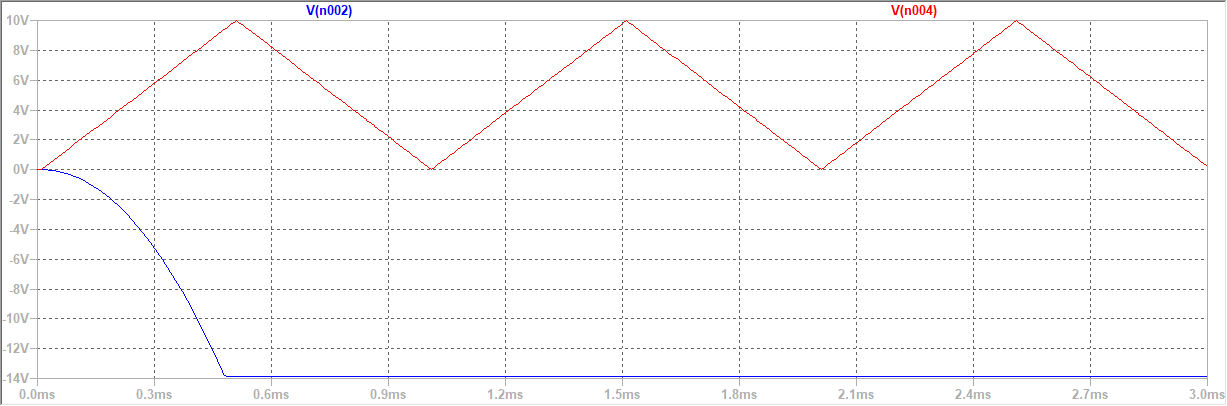
\includegraphics[scale=0.46]{3task_real_triangle.png}
        \captionsetup{skip=0pt}
        \caption{Треугольный сигнал, реальный интегратор}
        \label{fig:3task_real_triangle}
    \end{figure}
    \begin{figure}[H]
        \centering
        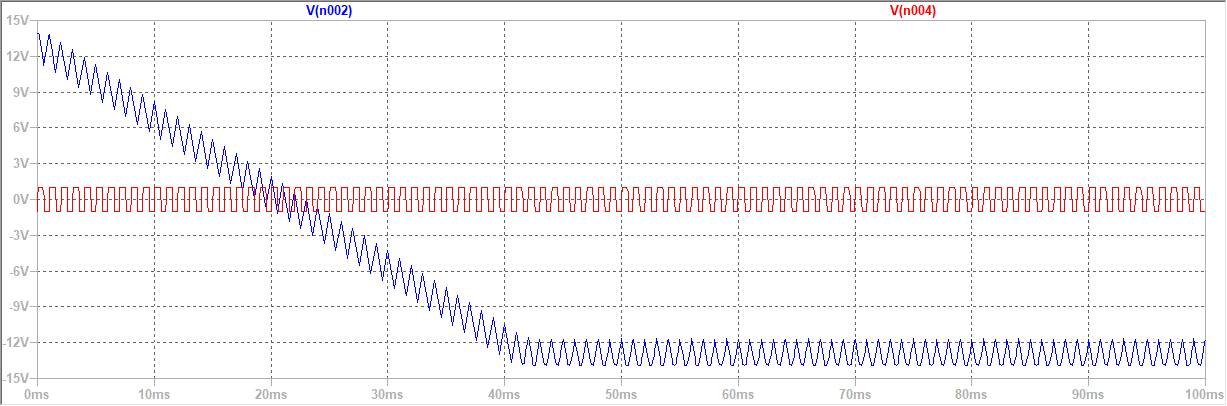
\includegraphics[scale=0.46]{3task_ideal_rect.png}
        \captionsetup{skip=0pt}
        \caption{Прямоугольный сигнал, идеальный интегратор}
        \label{fig:3task_ideal_rect}
    \end{figure}
    \begin{figure}[H]
        \centering
        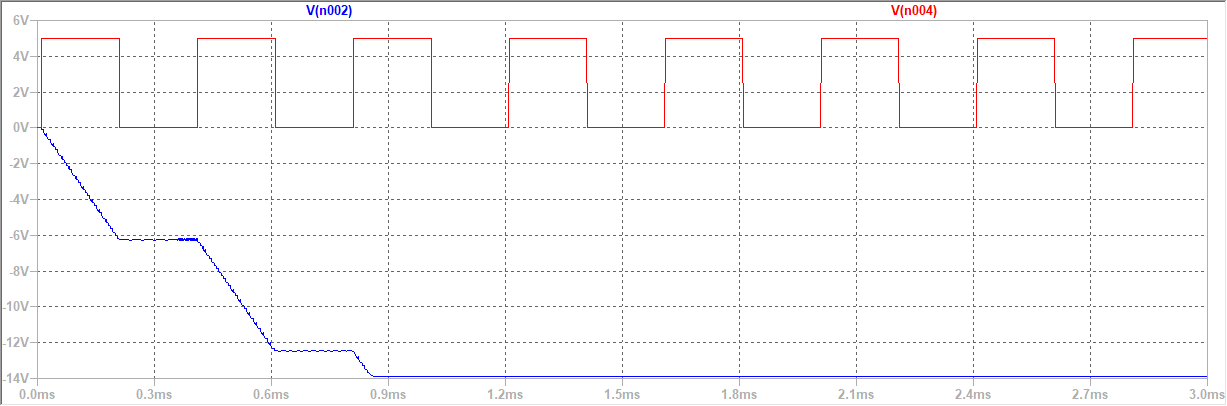
\includegraphics[scale=0.46]{3task_real_rect.png}
        \captionsetup{skip=0pt}
        \caption{Прямоугольный сигнал, реальный интегратор}
        \label{fig:3task_real_rect}
    \end{figure}
    \noindent Синусоидальный сигнал превратился в косинусоидальный выход, треугольный в параболический,
    прямоугольный в треугольный. Результаты подтверждают, что ОУ неинвертирующий.


    \section{Дифференциатор на ОУ}
    Соберем схему идеального дифференциатора на ОУ (см. рис. \ref{fig:scheme10}). Определим значения
    параметров элементов схемы. Зададим значение резистора в цепи
    обратной связи $R_2=50$ кОм. Вычислим соответствующее значение емкости
    при $f_d=1$ кГц
    $$
    C=\dfrac{1}{2\pi f_d R_2}=\dfrac{1}{2\pi\cdot10^3\cdot50\cdot10^3}=3.2\text{ нФ}
    $$
    Пусть минимальная рабочая частота работы дифференциатора
    (частота, при которой коэффициент усиления равен единице)
    $$
    f_{min}=\dfrac{f_d}{10}=\dfrac{10^3}{10}=100\text{ Гц}
    $$


    Соберем также схему реального операционного усилителя (см. рис. \ref{fig:scheme11}). Рассчитаем параметры схемы.
    Пусть минимальная рабочая частота дифференциатора также будет в 10 раз меньше
    рабочей частоты $f_{min}=f_d/10=100$ Гц. Вычислим значение емкости конденсатора $C_1$
    $$
    C_1\geq\dfrac{1}{2\pi R_2f_{min}}=\dfrac{1}{2\pi\cdot50\cdot10^3\cdot10^2}=31.8\text{ нФ}
    $$
    Выберем максимальную частоту дифференциатора в 10 раз выше рабочей частоты
    $$
    f_{max}=10f_d=10\cdot10^3=10\text{ кГц}
    $$
    Вычислим значение сопротивления резистора $R_1$
    $$
    R_1\leq\dfrac{1}{2\pi C_1f_{max}}=\dfrac{1}{2\pi\cdot31.8\cdot10^{-9}\cdot10^4}=500.4872424273\text{ Ом}
    $$
    Примем $R_1=500$ Ом.


    \subsection{Схема идеального дифференциатора на ОУ}
    Построим схему идеального дифференциатора с учетом всех вычислений
    \begin{figure}[H]
        \centering
        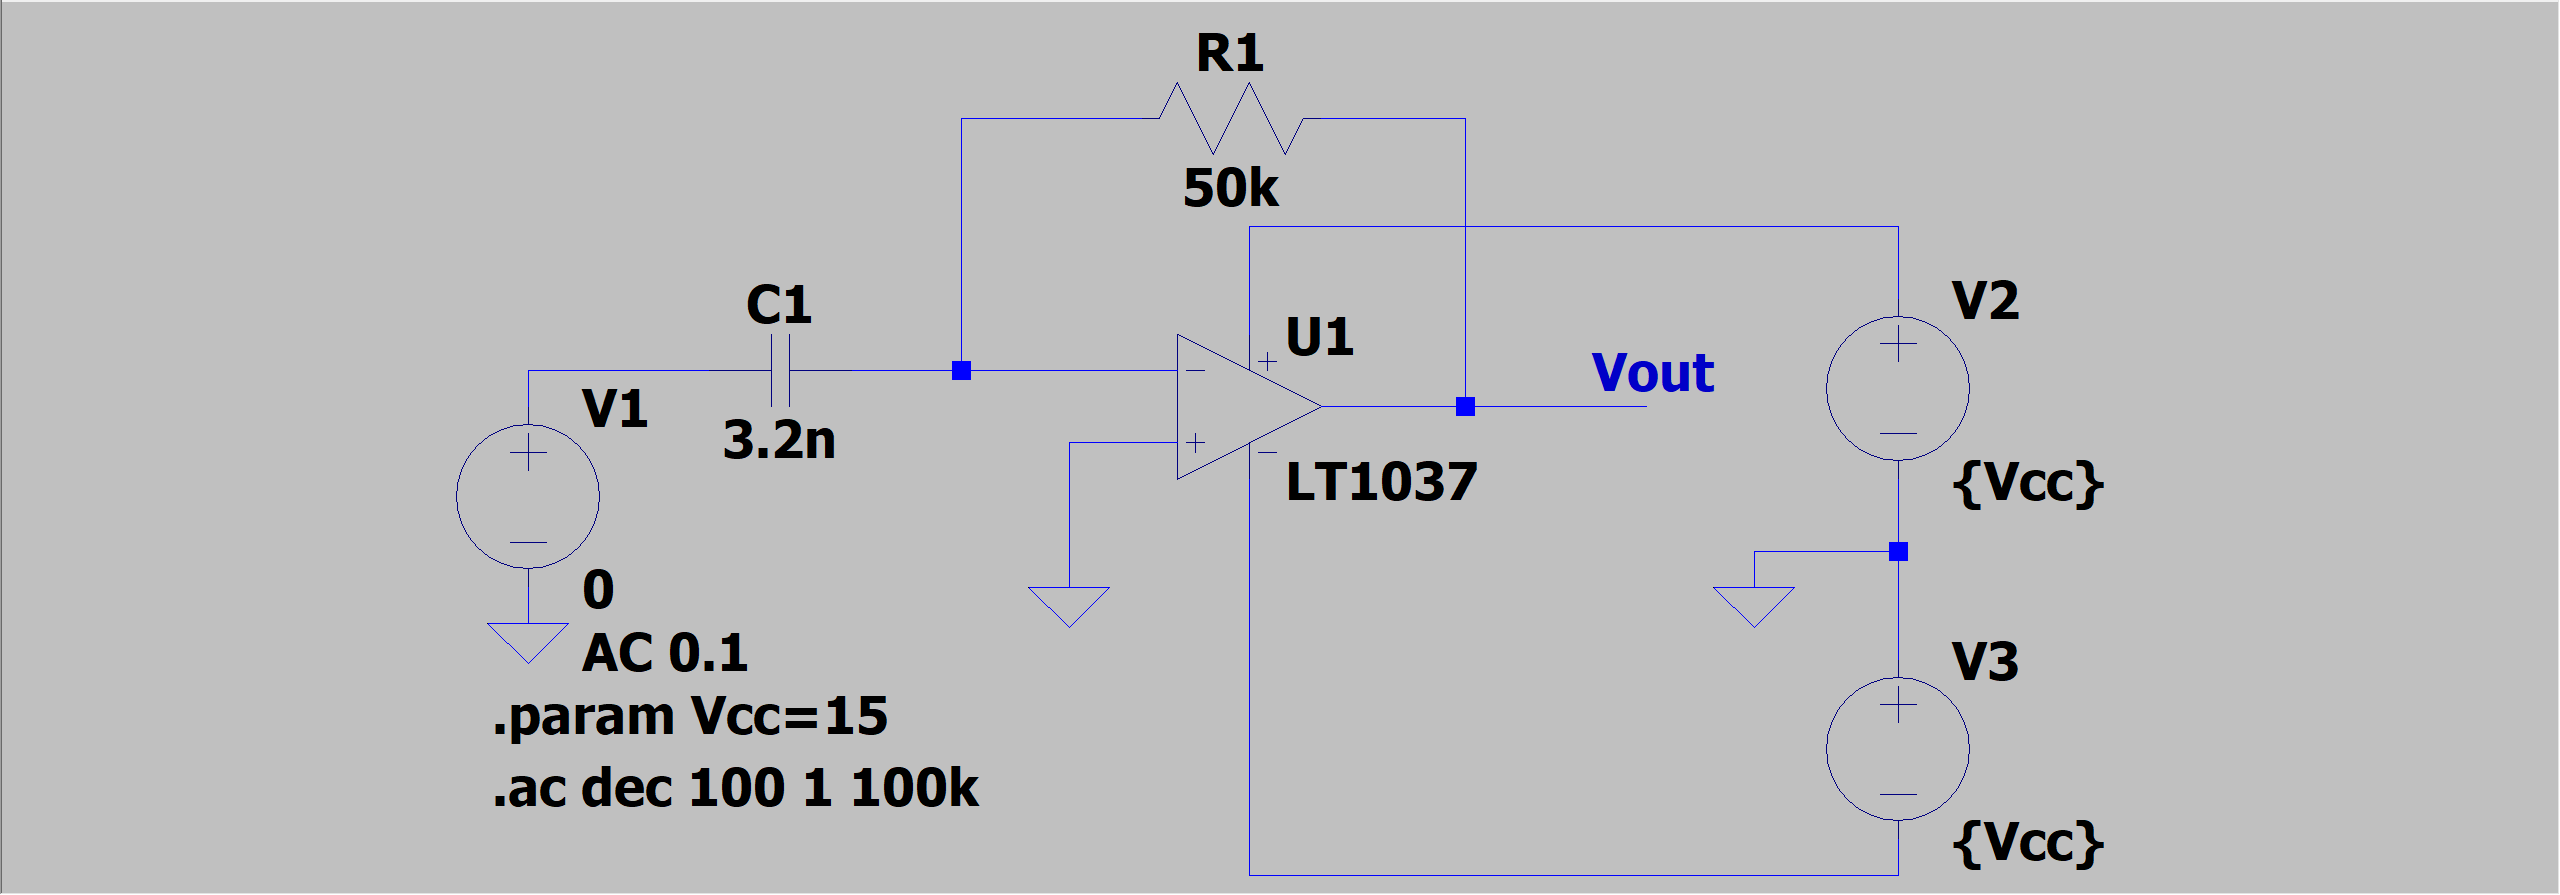
\includegraphics[scale=0.22]{scheme10.png}
        \captionsetup{skip=0pt}
        \caption{Идеальный дифференциатор на ОУ}
        \label{fig:scheme10}
    \end{figure}


    \subsection{Схема реального дифференциатора на ОУ}
    Построим схему реального дифференциатора с учетом всех вычислений
    \begin{figure}[H]
        \centering
        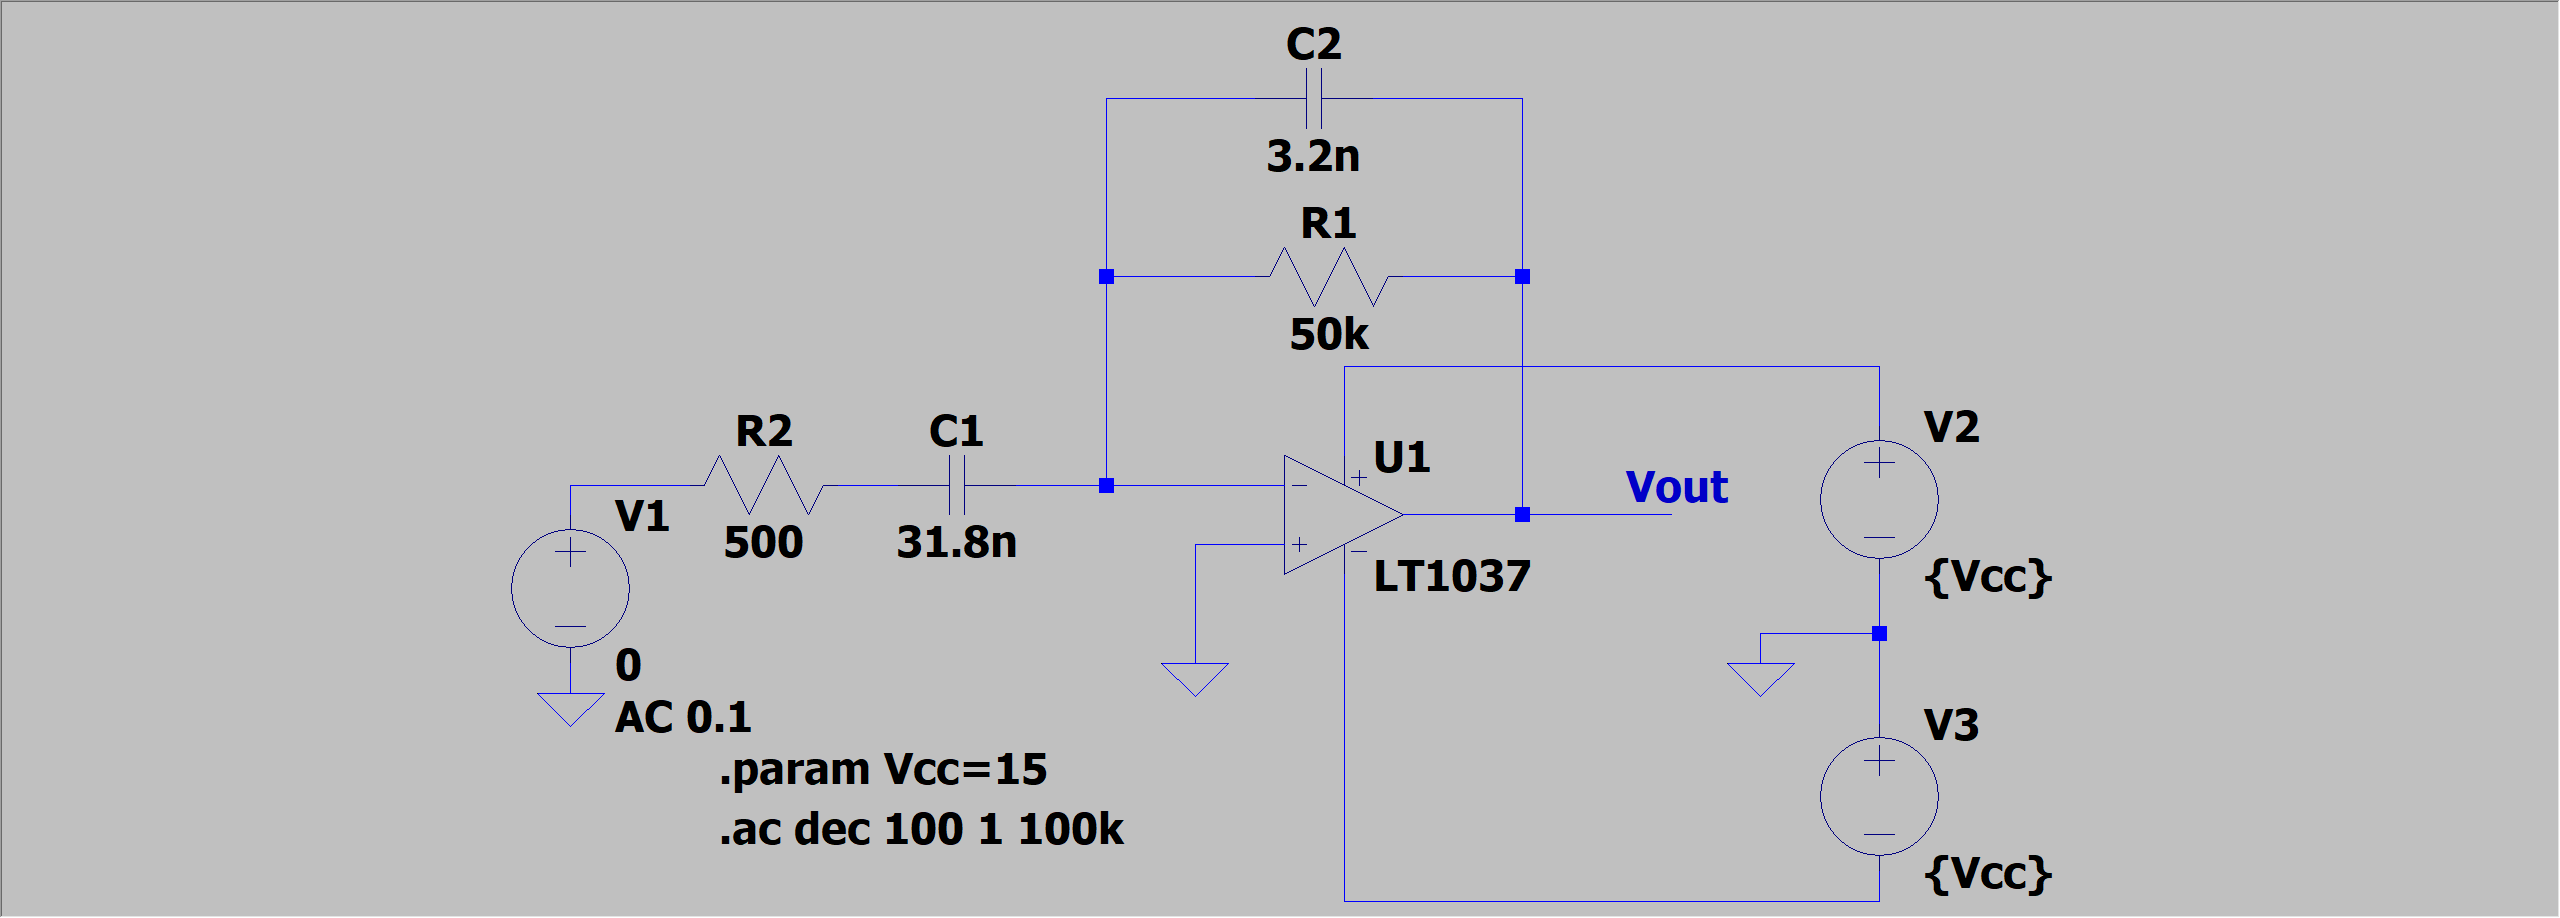
\includegraphics[scale=0.22]{scheme11.png}
        \captionsetup{skip=0pt}
        \caption{Реальный дифференциатор на ОУ}
        \label{fig:scheme11}
    \end{figure}


    \subsection{Частотная характеристика дифференциатора}
    Подадим на вход гармонический сигнал, не искажающий выходной сигнал (AC 0.1).
    Результаты для идеального дифференциатора представлены на рис. \ref{fig:4task_ideal_diff}, для
    реального \ref{fig:4task_real_diff}
    \begin{figure}[H]
        \centering
        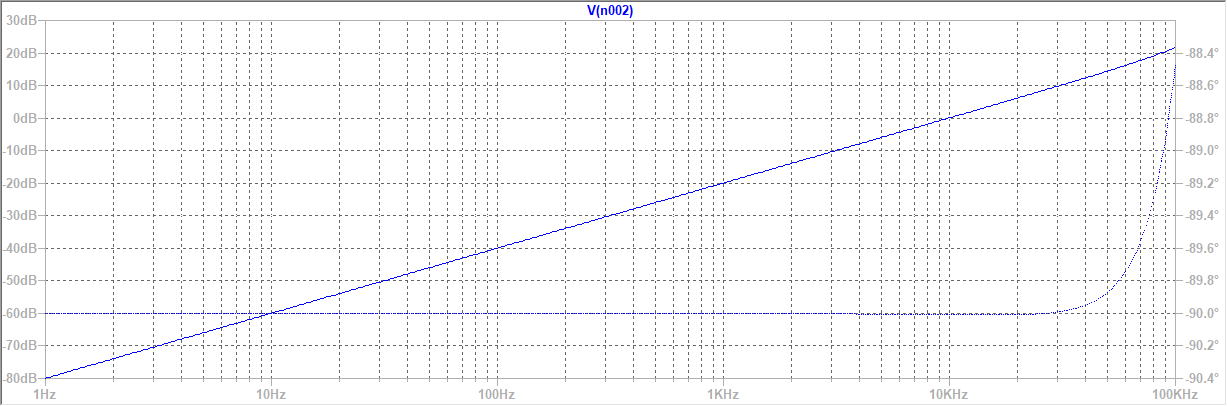
\includegraphics[scale=0.46]{4task_ideal_diff.png}
        \captionsetup{skip=0pt}
        \caption{Частотная характеристика идеального дифференциатора}
        \label{fig:4task_ideal_diff}
    \end{figure}
    \begin{figure}[H]
        \centering
        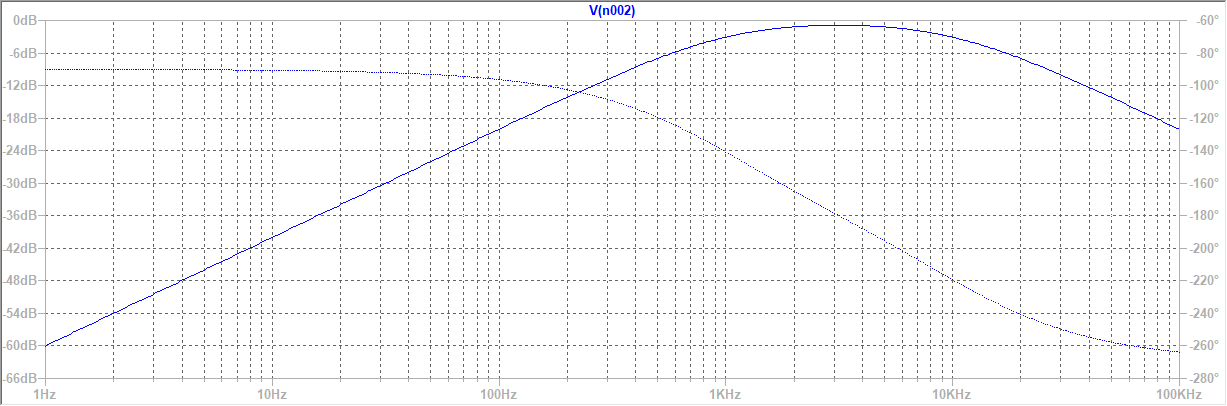
\includegraphics[scale=0.46]{4task_real_diff.png}
        \captionsetup{skip=0pt}
        \caption{Частотная характеристика реального дифференциатора}
        \label{fig:4task_real_diff}
    \end{figure}
    \noindent Посчитаем частоту среза ($C_2=C=3.2$ нФ)
    $$
    f_{\text{срез.}}=\dfrac{1}{2\pi C_2R_2}=\dfrac{1}{2\pi\cdot3.2\cdot10^{-9}\cdot50\cdot10^3}=994.7183943243\text{ Гц}\simeq 1\text{ кГц}
    $$
    То есть реальный дифференциатор перестает быть идеальным около 1 кГц, дальше его эффективность снижается.


    \subsection{Вид выходного сигнала при разных входных сигналах}
    Проверим экспериментально вид выходного сигнала аналогично пункту с интегратором.
    Результаты представлены на рис. \ref{fig:4task_ideal_sine}--\ref{fig:4task_real_rect}
    \begin{figure}[H]
        \centering
        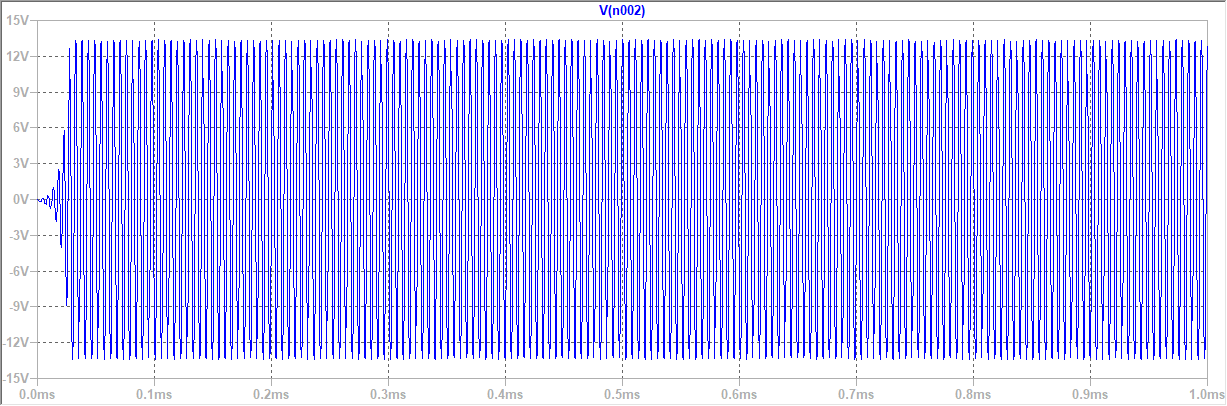
\includegraphics[scale=0.46]{4task_ideal_sine.png}
        \captionsetup{skip=0pt}
        \caption{Синусоидальный сигнал, идеальный дифференциатор}
        \label{fig:4task_ideal_sine}
    \end{figure}
    \begin{figure}[H]
        \centering
        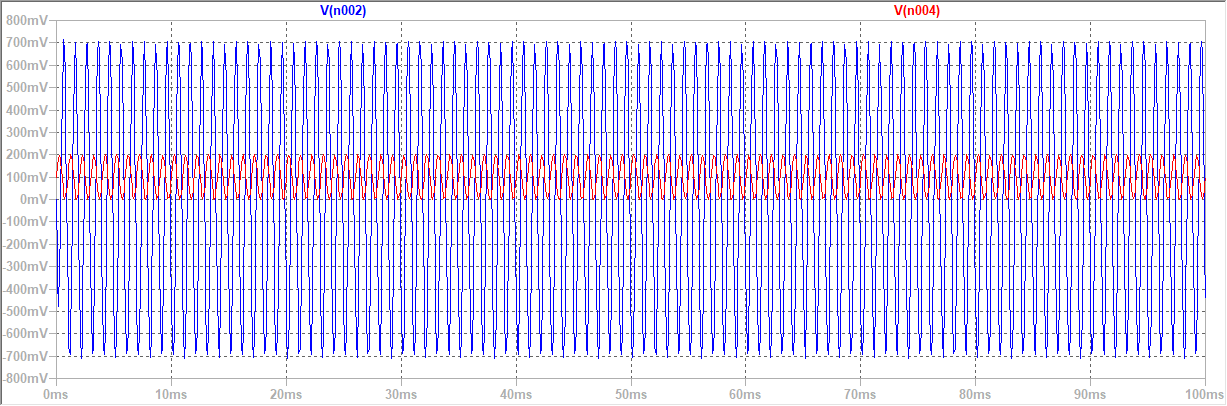
\includegraphics[scale=0.46]{4task_real_sine.png}
        \captionsetup{skip=0pt}
        \caption{Синусоидальный сигнал, реальный дифференциатор}
        \label{fig:4task_real_sine}
    \end{figure}
    \begin{figure}[H]
        \centering
        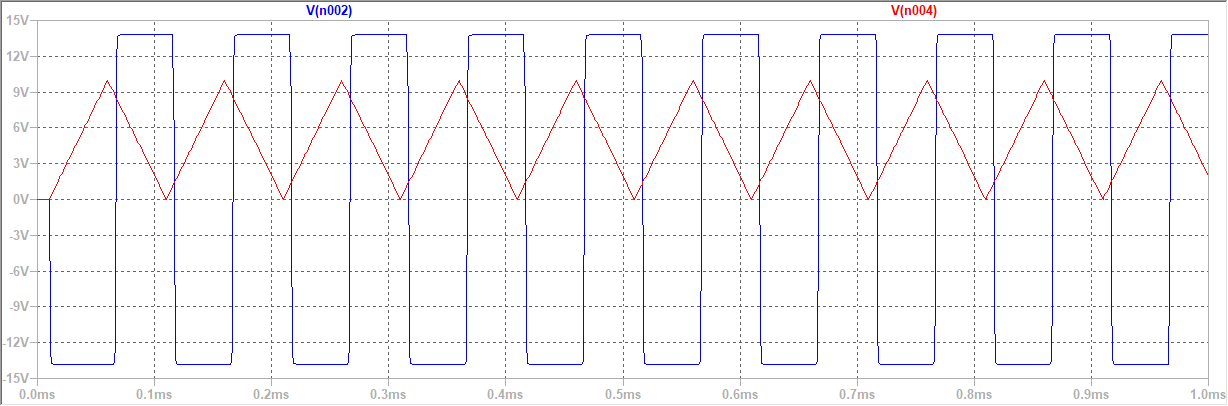
\includegraphics[scale=0.46]{4task_ideal_triangle.png}
        \captionsetup{skip=0pt}
        \caption{Треугольный сигнал, идеальный дифференциатор}
        \label{fig:4task_ideal_triangle}
    \end{figure}
    \begin{figure}[H]
        \centering
        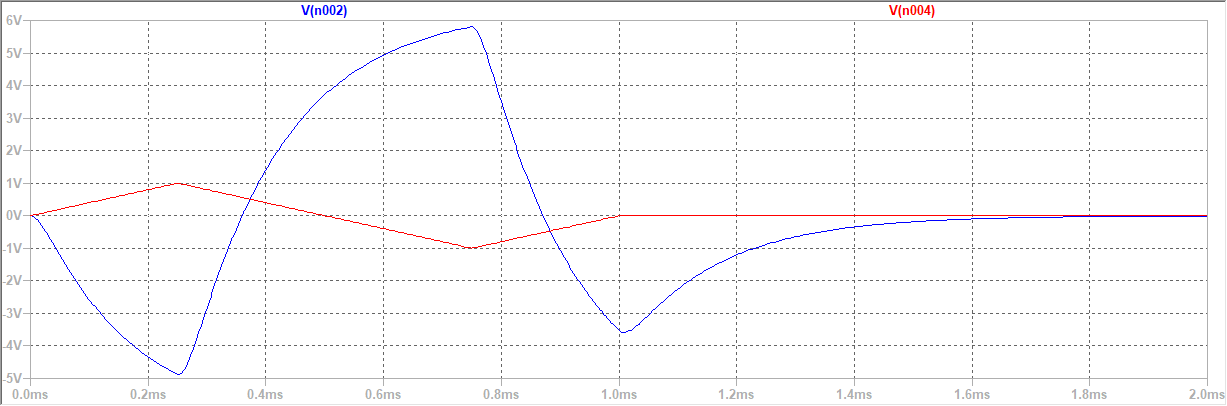
\includegraphics[scale=0.46]{4task_real_triangle.png}
        \captionsetup{skip=0pt}
        \caption{Треугольный сигнал, реальный дифференциатор}
        \label{fig:4task_real_triangle}
    \end{figure}
    \begin{figure}[H]
        \centering
        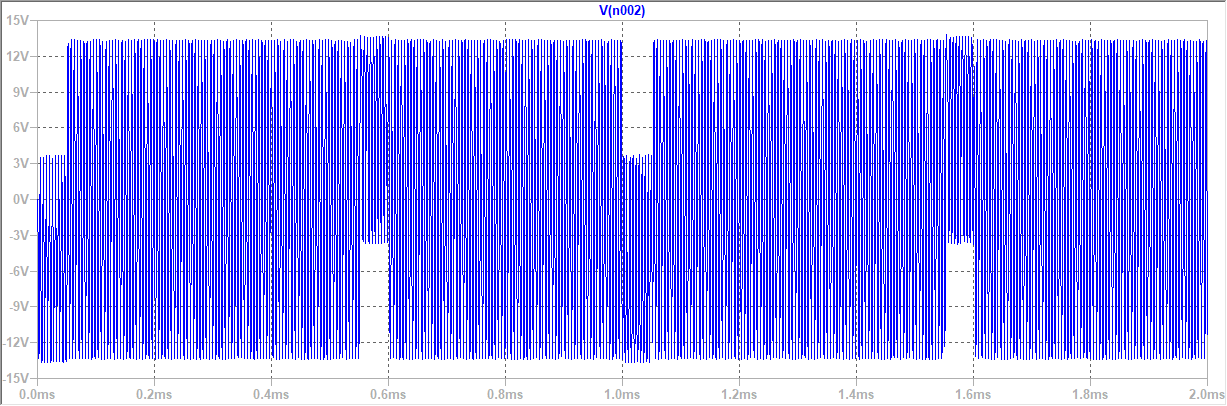
\includegraphics[scale=0.46]{4task_ideal_rect.png}
        \captionsetup{skip=0pt}
        \caption{Прямоугольный сигнал, идеальный дифференциатор}
        \label{fig:4task_ideal_rect}
    \end{figure}
    \begin{figure}[H]
        \centering
        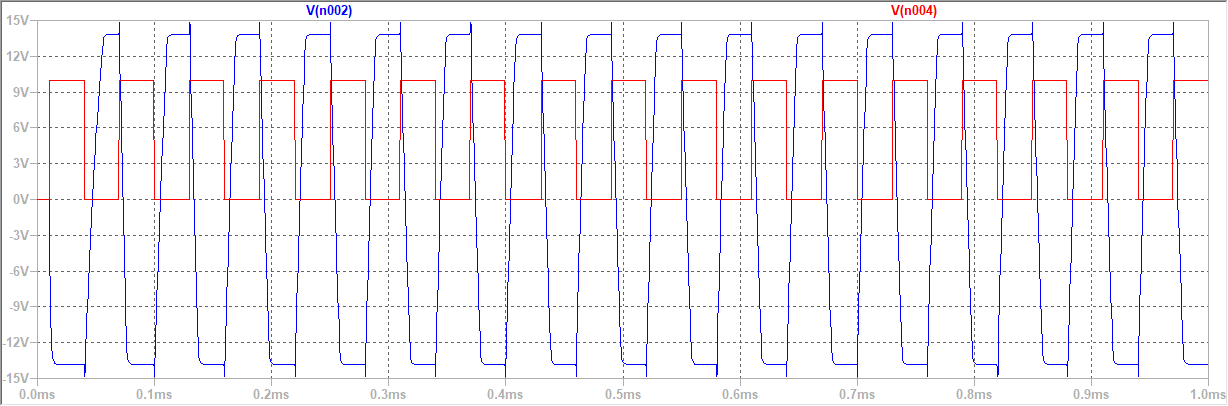
\includegraphics[scale=0.46]{4task_real_rect.png}
        \captionsetup{skip=0pt}
        \caption{Прямоугольный сигнал, реальный дифференциатор}
        \label{fig:4task_real_rect}
    \end{figure}


    \section{Вывод}
    В данной лабораторной работе были изучены различные схемы на операционных
    усилителях. Были исследованы дифференциальный усилитель, инвертирующий и
    неинвертирующий сумматоры, интегратор и дифференциатор. Для некоторых случаев
    было измерено выходное напряжение для различных входных напряжений.
    Были построены графики выходного напряжения при различных входных напряжениях, а
    для некоторых случаев были получены графики частотных характеристик сигнала.
\end{document}